
%% ----------------------------
%%  Make4ht: Plantilla para traducir LaTeX a html e insertar actividades interactivas con JavaScript
%% ----------------------------

%% PDFLaTeX se compila como usual.


%% .: Make4ht  Compilar en terminal .:

% make4ht  --utf8 -c config.cfg  -f html5   -d SitioWeb  plantilla.tex "mathml,svg,Gin-dim"



\documentclass[fleqn,oneside]{article}


%% ----------------------------
%% 1. CONFIGURACIÓN BÁSICA DEL DOCUMENTO
%% ----------------------------
\usepackage{mathtools}                  % Mejoras para matemáticas, incluye amsmath
                                        % va antes de abel, por conflictos inline con \int, \sum, etc.
\ifdefined\HCode
    \usepackage[spanish,english]{babel} % NO CAMBIAR: make4ht necesita english
    \usepackage[T1]{fontenc}            % Para fuentes con acentos correctamente
    \usepackage[utf8]{inputenc}         % Si usas LaTeX clásico
\else
    \usepackage[spanish,english, es-noquoting]{babel}
    \usepackage[autostyle, spanish = mexican]{csquotes} % Manejo de comillas
    \MakeOuterQuote{"}
    \usepackage[T1]{fontenc}
    \usepackage[utf8]{inputenc} % Para fuentes con acentos correctamente
    \decimalpoint % Cambiar a punto
\fi

%% ----------------------------
%%  "GEOMETRÍA" DE LA HOJA
%% ----------------------------
\RequirePackage[a4paper, top=2cm, bottom=2cm, left=2cm, right=2cm, headsep=10pt]{geometry}
%% ----------------------------
%%  PAQUETES BÁSICOS
%% ----------------------------
\RequirePackage{adjustbox}
\RequirePackage{changepage}                 % Ajuste de márgenes
\RequirePackage[table]{xcolor}
% Opciones para los caption
\RequirePackage[labelfont=bf,font=small]{caption}
% Cabeceras bonitas
\RequirePackage{fancyhdr}
% Comandos con opciones
\RequirePackage{xargs}
\RequirePackage{xparse}					% \NewDocumentEnvironment
% Tablas más bonitas
\RequirePackage{booktabs}
%Para opciones de los títulos de sección
\RequirePackage{titlesec}
%% ----------------------------
%%  HIPERVÍNCULOS Y REFERENCIAS
%% ----------------------------
\RequirePackage{hyperref}
%\usepackage{hyperref}                   % Hipervínculos
\definecolor{ligas}{HTML}{0000EE}       % Color para enlaces
\hypersetup{
    colorlinks=true,
    urlcolor=ligas,
    linkcolor=ligas,
    citecolor=ligas,
    hyperindex=true,
    linktoc=all
}
%% ----------------------------
%%  CONFIGURACIÓN DE TEXTO, FUENTES, ENUMERACION, CAPTION
%% ----------------------------
\ifdefined\HCode\else % fuentes PDFLATEX -> pdf
%\RequirePackage{pslatex}                              % Fuentes finas postscript
%\RequirePackage[sc]{mathpazo}                         % Fuentes mathpazo
\RequirePackage{palatino}
\RequirePackage{tgpagella}
%\RequirePackage{eulerpx}
\RequirePackage{eucal}
\RequirePackage[scaled=0.83]{beramono}
%\RequirePackage{chancery}
\RequirePackage{helvet}
\setlength{\parskip}{12pt} % El espacio en el HTML se definió en config.cfg
\fi
\parindent=0mm
\usepackage[fixed]{fontawesome5}        % Iconos modernos
\usepackage{longtable}
\usepackage{latexsym, stmaryrd}         % Símbolos matemáticos adicionales
\usepackage{amssymb, amsthm}   % Paquetes AMS estándar
%\let\openbox\relax % Eliminar el cuadrado al final de una prueba con "proof"
% proof
\renewcommand{\qedsymbol}{\textcolor{razul}{\rule{1.2ex}{1.2ex}}}




%----------------------------


\usepackage[labelfont=bf, font=small]{caption} % Configuración de caption
\usepackage{subcaption}                 % Subfiguras
%Redefinir itemize como enumerate con bullets
\usepackage{enumitem}

% Redefinir itemize para que sea enumerate con números
\let\olditemize\itemize
\let\oldenditemize\enditemize
\renewenvironment{itemize}{%
  \begin{enumerate}%
}{%
  \end{enumerate}%
}
%% ----------------------------
%%  COLORES
%% ----------------------------
\definecolor{nota}{rgb}{0.83, 0.18, 0.18}         % Rojo intenso (\#D32F2F)
\definecolor{fgray}{RGB}{251, 251, 251}
\definecolor{ffgray}{rgb}{.7,.7,.7}
\definecolor{blanco}{RGB}{255,255,255}
\definecolor{c666666}{RGB}{102,102,102}
\definecolor{ca7b1a6}{RGB}{167,177,166}
\definecolor{c100f0d}{RGB}{16,15,13}
% Color para los t\'itulos de las secciones y subsecciones
\definecolor{fazul}{RGB}{245, 245, 240}   % Azul original (0, 0, 153) con 5% de opacidad
\definecolor{razul}{RGB}{0,0,128}
\definecolor{azulEntornos}{rgb}{.0,.0,.3}
\definecolor{azulTitulos}{RGB}{37,74,165}
\definecolor{amarilloEntornos}{RGB}{248,248,245}
\definecolor{amarilloLema}{RGB}{255,202,0}
\definecolor{azulNota}{RGB}{68,0,170}
\definecolor{amarilloCaja}{RGB}{251,237,121}
\definecolor{fntGris}{rgb}{.3,.3,.3}
\definecolor{fntVerde}{RGB}{0,50,0}
\definecolor{tverde}{HTML}{176B3B}
\definecolor{torange}{HTML}{993C00}
\definecolor{headerblue}{RGB}{0, 82, 147}
\definecolor{rowgray}{RGB}{242, 242, 242}
\definecolor{highlight}{RGB}{255, 215, 0}
% Color para entornos (en este documento no se usan todos)
\definecolor{definicion}{rgb}{0.18, 0.49, 0.20}   % Verde oscuro (#2E7D32)
\definecolor{teorema}{rgb}{0.96, 0.49, 0.00}      % Naranja (#F57C00)
\definecolor{ejemplo}{rgb}{0.10, 0.46, 0.82}      % Azul fuerte (#1976D2)
\definecolor{nota}{rgb}{0.83, 0.18, 0.18}         % Rojo intenso (#D32F2F)
\definecolor{lema}{rgb}{1.00, 0.60, 0.00}         % Naranja claro (#FF9800)
\definecolor{corolario}{rgb}{0.98, 0.75, 0.18}    % Amarillo dorado (#FBC02D)
\definecolor{axioma}{rgb}{0.72, 0.11, 0.11}       % Rojo oscuro (#B71C1C)
\definecolor{conjetura}{rgb}{0.48, 0.12, 0.64}    % Morado (#7B1FA2)
\definecolor{problema}{rgb}{0.90, 0.32, 0.00}     % Naranja oscuro (#E65100)
\definecolor{casoespecial}{rgb}{0.40, 0.73, 0.42} % Verde claro (#66BB6A)
\definecolor{advertencia}{rgb}{0.78, 0.15, 0.15}  % Rojo fuerte (#C62828)
\definecolor{aplicacion}{rgb}{0.26, 0.65, 0.96}   % Azul celeste (#42A5F5)
\definecolor{historia}{rgb}{0.48, 0.34, 0.27}     % Marrón (#795548)
\definecolor{explicacionalt}{rgb}{0.00, 0.53, 0.48} % Verde azulado (#00897B)
\definecolor{referenciacruzada}{rgb}{0.26, 0.26, 0.26} % Gris oscuro (#424242)
\definecolor{proyecto}{rgb}{0.05, 0.28, 0.63}     % Azul oscuro (#0D47A1)
\definecolor{cita}{rgb}{0.98, 0.55, 0.00}         % Naranja suave (#FB8C00)
\definecolor{bibliografia}{rgb}{0.38, 0.38, 0.38} % Gris medio (#616161)
\definecolor{nota}{rgb}{0.83, 0.18, 0.18}         % Rojo intenso (\#D32F2F)
\definecolor{actividad}{rgb}{0.55, 0.83, 0.37}         % Rojo intenso (\#D32F2F)
%% ----------------------------
%% 5. ELEMENTOS GRÁFICOS
%% ----------------------------
\usepackage{tikz}                       % Gráficos vectoriales
\usetikzlibrary{matrix}                 % Funcionalidad adicional para TikZ
%\def\pgfsysdriver{pgfsys-dvisvgm4ht.def}% para responsividad html
\usepackage{adjustbox}                  % Ajuste de cajas
\usepackage{changepage}                 % Ajuste de márgenes
\usepackage{array, booktabs}            % Tablas profesionales
\usepackage{multirow}                   % Celdas multi-fila
\newcolumntype{P}[1]{>{\centering\arraybackslash}p{#1}} % Columna centrada
%% ----------------------------
%% PAQUETES ESENCIALES
%% ----------------------------
\usepackage{float}                      % Posicionamiento de figuras/tablas
\usepackage{lipsum}                     % Texto de relleno
\usepackage{multicol}                   % Múltiples columnas
\usepackage{iftex}                      % Detección del motor de compilación
\usepackage[numbers]{natbib}            % Bibliografía [1],[2]                     % Más opciones para comandos
\usepackage{environ}                    % Entornos personalizados
\usepackage{etoolbox}                   % Herramientas para programación
\usepackage{cancel}                     % Para tachar términos matemáticos
\usepackage{bbm}
\ifdefined\HCode % Paquete de ejercicios exsheets, actualmente no soportado por Make4ht, solo PDFLatex
\else %solo PDFLatex
\usepackage[counter-format=se.qu,counter-within=section]{exsheets}
\DeclareTranslation{english}{exsheets-exercise-name}{\textcolor{tverde}{Ejercicio}}
 \DeclareTranslation{english}{exsheets-question-name}{\textcolor{tverde}{Pregunta}}
 \DeclareTranslation{english}{exsheets-solution-name}{\textcolor{tverde}{Solución}}
\SetupExSheets{
	question/pre-body-hook = {\normalfont},
	solution/pre-hook = {\par\medskip},
}
\fi

%% ----------------------------
%% LISTADOS DE CÓDIGO: LISTINGS
%% ----------------------------
\RequirePackage{listings}
\lstset{captionpos=t}
\renewcommand{\lstlistingname}{C\'odigo} % Es importante el acento de esa manera

% Definir colores personalizados para listings
\definecolor{mauve}{rgb}{0.58,0,0.82}
\definecolor{codegreen}{rgb}{0,0.6,0}
\definecolor{codegray}{rgb}{0.5,0.5,0.5}
\definecolor{codepurple}{rgb}{0.58,0,0.82}
\definecolor{backcolour}{rgb}{0.99,0.99,0.99}
\definecolor{lstgray}{RGB}{251, 251, 251}
% Configuración del entorno listings
%\renewcommand{\ttdefault}{pcr}

\captionsetup[lstlisting]{%
  %font=small, % Hace que el texto del caption sea pequeño
  labelfont=bf, % Hace que el "Listado X" sea negrita
  %textfont=bf % Hace que el texto del caption sea negrita
  %justification=raggedright, % <--- Alinea el caption a la izquierda
  %singlelinecheck=false % Importante: asegura que se aplique incluso si es una sola línea
}
\lstset{
    language={[latex]TeX}, % Lenguaje LaTeX
    backgroundcolor=\color{backcolour}, % Color de fondo
    basicstyle=\small\fontseries{b}\ttfamily, % Estilo básico
    breakatwhitespace=false, % No romper líneas en espacios en blanco
    breaklines=true, % Romper líneas largas
    commentstyle=\color{mauve}, % Estilo de los comentarios
    %deletekeywords={...}, % Palabras clave a eliminar
    escapeinside={\%*}{*)}, % Escapar dentro del código
     extendedchars=true, % Caracteres extendidos
     frame=single, % Marco alrededor del código
    keepspaces=true, % Mantener espacios
     moredelim=[is][\color{red}]{\%*}{*\%}, % Delimitador personalizado
 keywordstyle=\color{blue}, % Estilo de las palabras clave
 morekeywords={*,usepackage,begin,end, lstinline, newenvironment,
 	tabular, minipage, pmatrix,bmatrix, includegraphics,captionof,width,scale,rowcolor,multirow,multicolumn, documentclass, input,ifdefined, HCode,Configure,fi, ConfigureEnv,insertarhtml, ifvmode,label,Css,pdfomk,ejersol,hejersol},
    texcsstyle=[1]\color{blue},%label, caption, etc.
     numbers=none,
     %numbers=left, % Números de línea a la izquierda
     %numbersep=5pt, % Separación de los números de línea
     %numberstyle=\tiny\color{codegray}, % Estilo de los números de línea
     rulecolor=\color{gray}, % Color de la regla
     showspaces=false, % No mostrar espacios
     showstringspaces=false, % No mostrar espacios en cadenas
     showtabs=false, % No mostrar tabulaciones
     %stepnumber=1, % Paso de los números de línea
     stringstyle=\color{mauve}, % Estilo de las cadenas
     % NO Habilitar title=\lstname
     literate= {∩}{{$\cap$}}1 {á}{{\'a}}1 {é}{{\'e}}1 {í}{{{\'\i}}}1 {ó}{{\'o}}1 {ö}{{\"o}}1 {ő}{{\H o}}1 {ú}{{\'u}}1 {Ú}{{\'U}}1 {ü}{{\"u}}1 {ű}{{\H u}}1 {Ü}{{\"U}}1
}
%%--listing

%% ----------------------------
%% FUENTES PERSONALIZADAS
%% ----------------------------
\newcommand{\htmlusefont}[1]{% Make4ht -> html
  \HCode{<span class="ptsansnarrow">}#1\HCode{</span>}%
}
\newcommand{\fhvb}[2]{{\fontfamily{phv}\fontseries{b}\fontsize{#1}{1}\selectfont{#2}}}
\newcommand{\fhv}[2]{{\fontfamily{phv}\fontsize{#1}{1}\selectfont{#2}}}
\newcommand{\fvnp}[1]{\fhvb{10}{#1}}
\newcommand{\fte}[1]{\fhvb{10}{\textcolor{razul}{#1}}}
\newcommand{\fvn}[1]{\fhv{10}{#1}}
\newcommand{\fvns}[1]{\fhv{10}{#1}}
\newcommand{\fvntt}[1]{\fhv{10}{#1}}
\newcommandx{\fntg}[4][1=pag,2=9,3=n]{{\color{fntGris}\fontfamily{#1}\fontsize{#2}{1}\fontshape{#3}\selectfont{#4}}}
\newcommandx{\fnte}[4][1=phv,2=9,3=n]{{\color{fntVerde}\fontfamily{#1}\fontsize{#2}{1}\fontshape{#3}\selectfont{#4}}}
\newcommand{\ofvnp}[1]{\textcolor{torange}{\fvnp{#1}}}
\renewcommand{\tt}[1]{\textcolor{tverde}{\fvntt{#1}}}
\newcommand{\wtt}[1]{\textcolor{torange}{\fvntt{#1}}}
%--------------------------


%%-- TITULO - FECHA - AUTORES - RESUMEN - ABSTRACT - KEYWORDS - etc.
%--------------------------------------------------------------------------
%.: Título PDFLatex :.
\newcommand{\titulo}[6]{%espanol-ingl\'es-volumen-n\'umero-mes de inicio[, anno]-mes final, anno
	\title{
		\thispagestyle{empty}
		\headerInicial{Vol\; #3, \;No #4.   #5\,-\,#6}
		\begin{center}
			{\Large\bfseries #1}\\[0.22cm]
			{\usefont{T1}{PTSansNarrow-TLF}{}{n} | {\normalsize #2} |}
		\end{center}
		% Habilita las cabeceras en las páginas (con ese dise\~no)
		\revistaheaderA{Vol\; #3,\;No \;#4.  #5\,-\,#6}
		\medskip
	}
}
\newcommand{\headerInicial}[1]{
	\vspace{-2cm}
	\textcolor{lightgray}{\rule[0.5cm]{\textwidth}{4pt}}\\[-0.2cm]
	\begin{minipage}{0.1\textwidth}
		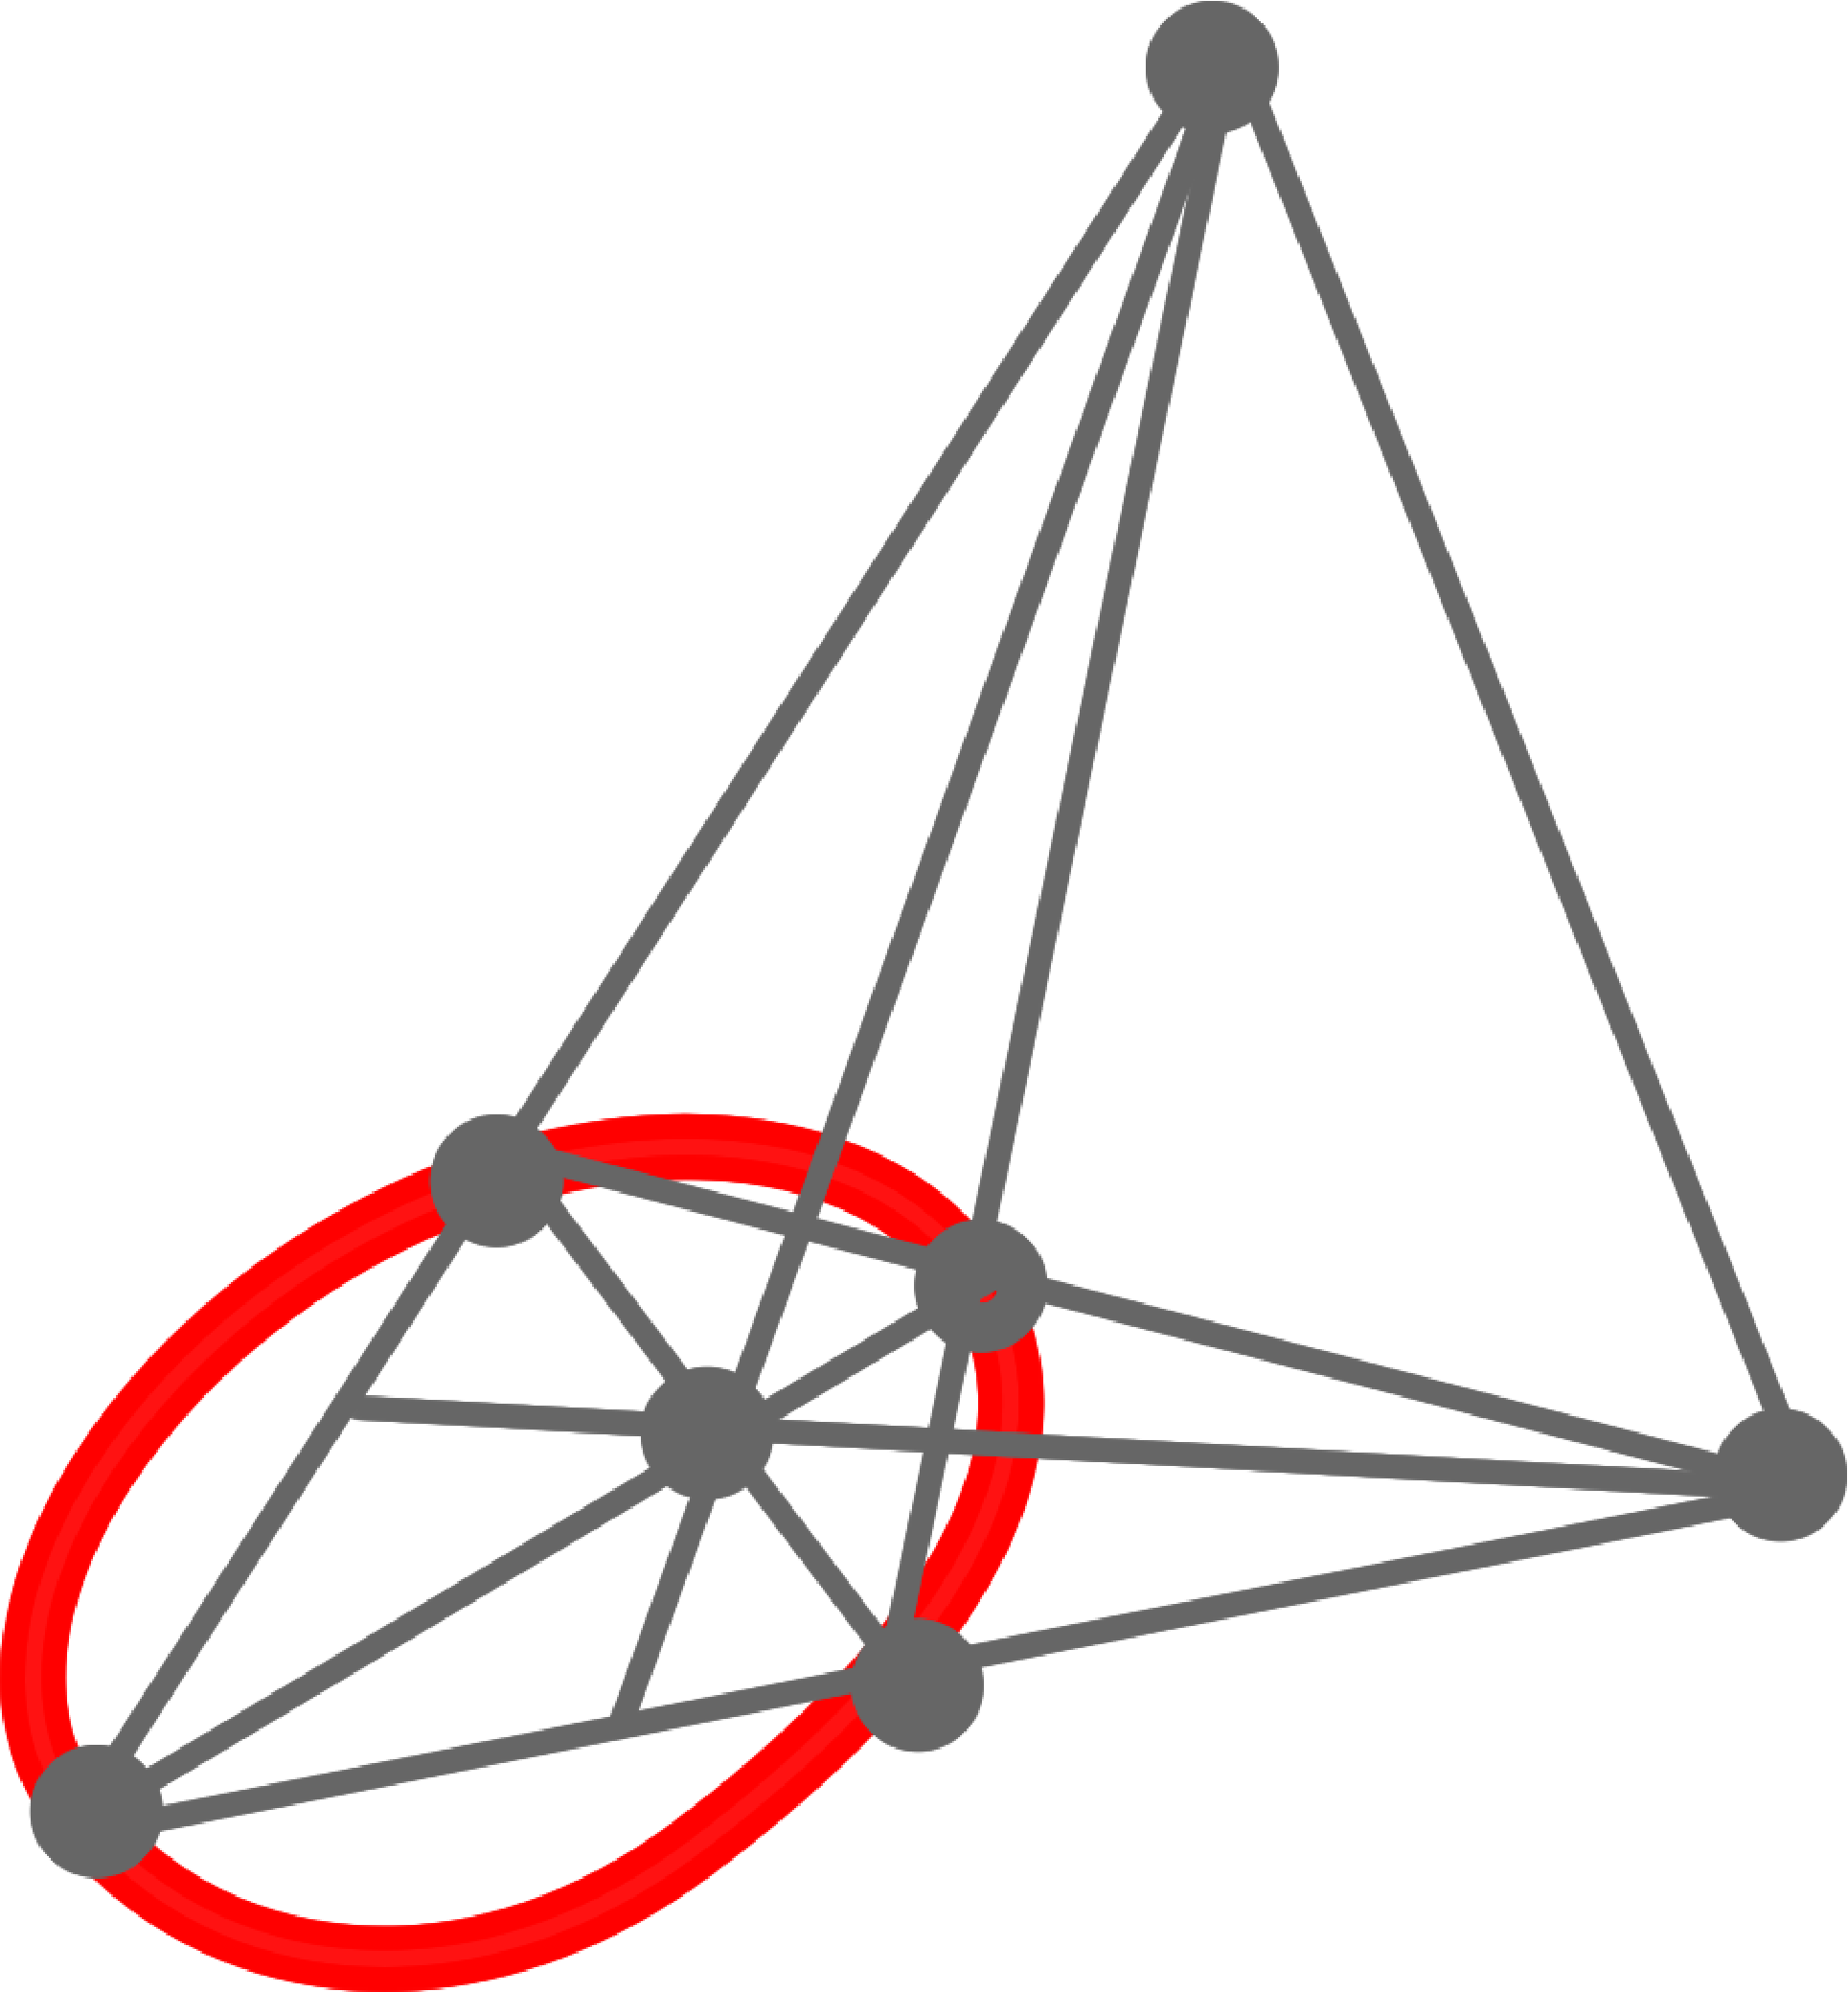
\includegraphics[width=1.4cm]{images/logo}
	\end{minipage}
	\begin{minipage}{0.85\textwidth}
		\fhv{10}{Revista digital }\\[-0.3cm]
		\fhvb{10}{Matem\'atica, Educaci\'on e Internet\hfill \fntg[phv][8]{
\includegraphics[scale=0.8]{images/logocc.png}}\\[-0.3cm]
			\fvn{%
				\href{https://revistas.tec.ac.cr/index.php/matematica}{https://revistas.tec.ac.cr/index.php/matematica}}\hfill \fntg[phv][8]{ISSN 1659 -0643}}\\[-0.3cm]
		\fvn{#1} \hfill \fntg[phv][8]{DOI: \href{https://doi.org/10.18845/rdmei.v26i2.8214}{10.18845/rdmei.v26i2.8214}}
	\end{minipage}
	\textcolor{lightgray}{\rule[0.5cm]{\textwidth}{0.1pt}}
}
%\revistaheaderA{V\lowercase{ol 12, }N\lowercase{o 2. }  M\lowercase{arzo} $-$ A\lowercase{gosto} 2012.}
 \newcommand{\revistaheaderA}[1]{\markboth{R\lowercase{evista digital} M\lowercase{atem\'atica,} E\lowercase{ducaci\'on e} I\lowercase{nternet} \lowercase{\href{https://revistas.tec.ac.cr/index.php/matematica}{\lowercase{(https://revistas.tec.ac.cr/index.php/matematica)}}}. #1}{R\lowercase{evista digital} M\lowercase{atem\'atica,} E\lowercase{ducaci\'on e}I\lowercase{nternet} \lowercase{\href{https://revistas.tec.ac.cr/index.php/matematica}{\lowercase{(https://revistas.tec.ac.cr/index.php/matematica)}}}. #1}}


%--------------------------------------------------------------------------
%% .: TITULO para Make4ht :.
%-------------------------------------------------------------------------
\newcommand{\webtitulo}[6]{%espanol-ingl\'es-volumen-n\'umero-mes de inicio[, anno]-mes final, anno
{ %\begingroup necesario
\setlength{\arrayrulewidth}{6pt}
\arrayrulecolor{lightgray}
%\begin{tabular*}{\textwidth}{@{\extracolsep{\fill}}llr@{}}
\begin{tabular}{@{\extracolsep{\fill}}llr@{}}
\toprule[4pt]
        % --- Primera fila (autores 1, 2, 3) ---
        \begin{efntabular}
        \begin{tabular}[t]{@{}r@{}}
\raisebox{\dimexpr-\height + 1.5ex\relax}{  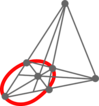
\includegraphics{images/weblogo.png}}
        \end{tabular}%
        \end{efntabular}
            &
            \begin{efntabular}
            \begin{tabular}[t]{@{}l@{}}
    \fhv{10}{Revista digital }\\
    \fhvb{10}{Matem\'atica, Educaci\'on e Internet}\\
    \fntg[phv][9]{\href{https://revistas.tec.ac.cr/index.php/matematica}{https://revistas.tec.ac.cr/index.php/matematica}}\\
    \fhv{10}{Vol\; #3,\;No \;#4.  #5 \,\textminus\,   #6}%\\
            \end{tabular}%
            \end{efntabular}
                &
                \begin{efntabular}
                \begin{tabular}[t]{@{}r@{}}
             \raisebox{\dimexpr-\height + 1.5ex\relax}{ 
\includegraphics{images/weblogocc.png}}\\
    \fntg[phv][8]{ISSN 1659 -0643}\\
   \fntg[phv][8]{DOI: \href{https://doi.org/10.18845/rdmei.v26i2.8214}{10.18845/rdmei.v26i2.8214}}\\
                \end{tabular}%
                \end{efntabular}\\
                \bottomrule
\end{tabular}
}
		\begin{center}
			{\Large\bfseries #1}\\
			\htmlusefont{| #2 |}
		\end{center}
    } % webtitulo

%--------------------------------------------------------------------------
%%-- Recibido - Aceptado
%-------------------------------------------------------------------------
\newcommand{\fecha}[2]{% PDFLaTeX -> pdf
	\date{
		{\textcolor{lightgray}{\rule[0.5cm]{0.8\textwidth}{0.1pt}}} \\[-0.2cm]
		\begin{minipage}{0.6\textwidth}
			\fhv{9}{\color{azulEntornos} Recibido: #1}\hfill\fhv{9}{\color{azulEntornos} Aceptado: #2}  \\[0.04cm]
			{\textcolor{lightgray}{\rule[0.5cm]{\textwidth}{0.1pt}}}
		\end{minipage}
		\vspace{-5mm}
	}
}
\newcommand{\webfecha}[2]{%
  \ifvmode\IgnorePar\fi\EndP
  { % grupo local
   \arrayrulecolor{lightgray}%
   \setlength{\arrayrulewidth}{0.3pt}%
   \begin{tabular*}{\textwidth}{@{\extracolsep{\fill}} p{0.3\textwidth} p{0.4\textwidth} p{0.3\textwidth} }
   \hline
      \HCode{<span style="color:\#1b3a75;">}\fvns{Recibido: #1}\HCode{</span>}
      &\HCode{<span style="display:inline-block; width: 4em;"></span>} & %espacio en la columna 2
      \HCode{<span style="color:\#1b3a75;">}\fvns{Aceptado: #2}\HCode{</span>} \\
    \cline{1-1} \cline{3-3}
  \end{tabular*}
  }
}


% Comando \cejilla
% ═══════════════════════════════════════════════════════════
% CEJILLA - Comando LaTeX para pestañas colapsables
% Uso: \cejilla{nombre}{contenido latex}
% ═══════════════════════════════════════════════════════════

% \newcommand{\webtableofcontents}{%
% \ifvmode\IgnorePar\fi\EndP
% \ifdefined\HCode
% \ifvmode\IgnorePar\fi\EndP
% \ifvmode\IgnorePar\fi\EndP
% \fi
% \ifdefined\HCode
% \ifvmode\IgnorePar\fi\EndP
% \tableofcontents
% \ifvmode\IgnorePar\fi\EndP
% \fi
% \ifdefined\HCode
% \ifvmode\IgnorePar\fi\EndP
% \HCode{</div>}
% \ifvmode\IgnorePar\fi\EndP
% \fi
% }

%% ----------------------------
%% COMANDOS ESPECIALES MAK4HT -> HTML
%% ----------------------------

%1.) Tablas hover...PDFLatex ignora,
%    Make4ht lo aplica:Una envoltura <div class="tabla-hover-filas">...
\newenvironment{tablahoverfilas}
  {%
    \ifdefined\HCode
      \ifvmode\IgnorePar\fi\EndP
      \HCode{<div class="tabla-hover-filas">}%
      \par
    \fi
  }
  {%
    \ifdefined\HCode
      \ifvmode\IgnorePar\fi\EndP
      \HCode{</div>}%
      \par
    \fi
  }
%
% \rowcolor{rowgray} tapa el hover, \rowgris para css y da \rowcolor{rowgray} para pdf
\ifdefined\HCode
  \newcommand{\rowgris}{\HCode{<tr class="rowgray">}}
\else
  \newcommand{\rowgris}{\rowcolor{rowgray}}
\fi
%%--
%2.) \vspace \bigskip, \medskip, \smallskip para html

\newcommand{\linea}{\textcolor{lightgray}{\rule{\linewidth}{0.4pt}}\par}
\ifdefined\HCode
  \def\bigskip{\HCode{<div style="margin-top:2em;"></div>}}
  \def\medskip{\HCode{<div style="margin-top:1.5em;"></div>}}
  \def\smallskip{\HCode{<div style="margin-top:1em;"></div>}}
  \def\linea{\HCode{<hr style="height:1px; border:none; background-color:\#ccc; margin:20px 0;">}}
\fi
%
\ifdefined\HCode
  \newcommand{\vspacehtml}[1]{\HCode{<div style="margin-top:#1;"></div>}}
\else
  \newcommand{\vspacehtml}[1]{\vspace*{#1}}
\fi
%% \vspacehtml{1em}
%%--
% 3.) Comandos \pdfomk{#1}{#2} e \insertarhtml{}

\ifdefined\HCode
  \long\def\solopdf#1{\protect}  % ignorado por make4ht
  \long\def\solomk#1{\protect#1} % procesado en make4ht
\else
  \long\def\solopdf#1{\protect#1} % procesado en PDF
  \long\def\solomk#1{\protect}    % ignorado por PDF
\fi

% 3a.) \pdfomk{#1}{#2}
\ifdefined\HCode
\long\def\pdfomk#1#2{%
	\protect#2%html
}
\else
\long\def\pdfomk#1#2{%
	\protect#1%pdf
}
\fi
%-3b.)--Insertar html
%
%--\insertarhtml{#1} %Para html PURO
  \ifdefined\HCode
    \long\def\insertarhtml#1{%
      \HCode{#1}%
    }
  \else
    \long\def\insertarhtml#1{%
      %nada%\textbf{[Contenido interactivo no disponible en PDF]}
    }
  \fi
%
%- 4.) Un entorno para ejercicio con botón para ver/ocultar respuesta
%
\newcounter{htmlEjercicio}[section]
\renewcommand{\thehtmlEjercicio}{%
  \ifnum\value{section}=0
    \arabic{htmlEjercicio}%
  \else
    \thesection.\arabic{htmlEjercicio}%
  \fi
}
% Nota: Debemos poner \insertarhtml{<script src="js/ejerciciosolucion.js" defer></script>}
% antes de \end{document}
% para que el script quede al  final del documento (justo antes de cerrar </body>),
% así todos los elementos HTML ya han sido parseados y existen en el DOM.
% Por lo tanto, document.querySelectorAll(".ejercicio-solucion button") puede encontrar
% los botones correctamente.
% \insertarhtml{<script src="js/ejerciciosolucion.js" defer></script>}
\ifdefined\HCode
\newcommand{\hejersol}[2]{%
    \stepcounter{htmlEjercicio}%
    \par\medskip
        \ifvmode\IgnorePar\fi\EndP
    \noindent\textbf{Ejercicio \thehtmlEjercicio}
    #1%
        \ifvmode\IgnorePar\fi\EndP
    \HCode{%
      <div class="ejercicio-solucion">
        <div class="solucion-container">
          <button onclick="this.nextElementSibling.classList.toggle('visible')">Mostrar/Ocultar solución</button>
          <div class="solucion">
          %<script src="js/ejerciciosolucion.js"></script>
    }%
        \ifvmode\IgnorePar\fi\EndP
    #2%
        \ifvmode\IgnorePar\fi\EndP
    \HCode{</div></div></div>}%
    \par\medskip
  }
\else
  \newcommand{\hejersol}[2]{%
    % No imprimir nada en PDF
  }
\fi
%%-- pdf-exsheet y make4ht
% Definición base para PDF (LaTeX estándar)
\newcommand{\ejersol}[2]{%[4][]{%  % #1 = opciones para question (opcional)
    \begin{question}%[#1]%
        #1%                    % #3 = enunciado
    \end{question}%
    \begin{solution}%[print=true]%  % Opción FIJADA para evitar errores
        #2%                    % #4 = solución
    \end{solution}%
}

% Sobrescribir para make4ht (HTML)
\ifdefined\HCode
    \renewcommand{\ejersol}[2]{\hejersol{#1}{#2}}  % Ignora opciones en HTML
\fi


%%------------------------------
% .: TABLA AUTORES PDFLATEX - MAKE4HT
%%-------------------------------

\newcommand{\autor}[5]{% Nombre - email - Universidad - Pa\'is - N\'umero de ORCID
	\def\nombreautoruno{#1}
	\def\correoautoruno{#2}
	\def\universidadautoruno{#3}
	\def\paisautoruno{#4}
	\def\orcidautoruno{#5}
}

\newcommand{\autordos}[5]{% Nombre - email - Universidad - Pa\'is - N\'umero de ORCID
	\def\nombreautordos{#1}
	\def\correoautordos{#2}
	\def\universidadautordos{#3}
	\def\paisautordos{#4}
	\def\orcidautordos{#5}
}

\newcommand{\autortres}[5]{% Nombre - email - Universidad - Pa\'is - N\'umero de ORCID
	\def\nombreautortres{#1}
	\def\correoautortres{#2}
	\def\universidadautortres{#3}
	\def\paisautortres{#4}
	\def\orcidautortres{#5}
}

\newcommand{\autorcuatro}[5]{% Nombre - email - Universidad - Pa\'is - N\'umero de ORCID
	\def\nombreautorcuatro{#1}
	\def\correoautorcuatro{#2}
	\def\universidadautorcuatro{#3}
	\def\paisautorcuatro{#4}
	\def\orcidautorcuatro{#5}
}

\newcommand{\autorcinco}[5]{% Nombre - email - Universidad - Pa\'is - N\'umero de ORCID
	\def\nombreautorcinco{#1}
	\def\correoautorcinco{#2}
	\def\universidadautorcinco{#3}
	\def\paisautorcinco{#4}
	\def\orcidautorcinco{#5}
}

\newcommand{\autorseis}[5]{% Nombre - email - Universidad - Pa\'is - N\'umero de ORCID
	\def\nombreautorseis{#1}
	\def\correoautorseis{#2}
	\def\universidadautorseis{#3}
	\def\paisautorseis{#4}
	\def\orcidautorseis{#5}
}

\newcommand{\autorsiete}[5]{% Nombre - email - Universidad - Pa\'is - N\'umero de ORCID
	\def\nombreautorsiete{#1}
	\def\correoautorsiete{#2}
	\def\universidadautorsiete{#3}
	\def\paisautorsiete{#4}
	\def\orcidautorsiete{#5}
}

\newcommand{\autorocho}[5]{% Nombre - email - Universidad - Pa\'is - N\'umero de ORCID
	\def\nombreautorocho{#1}
	\def\correoautorocho{#2}
	\def\universidadautorocho{#3}
	\def\paisautorocho{#4}
	\def\orcidautorocho{#5}
}

\newcommand{\autores}{% Nombre - email - Universidad - Pa\'is - N\'umero de ORCID
	\author{
		\fnte[phv][12]{\href{https://orcid.org/\orcidautoruno}{
\includegraphics[scale=0.65]{./images/ORCID-iD_icon-16x16.png}} \nombreautoruno}\\
		\fvn{\correoautoruno}\\
		\fvn{\universidadautoruno} \\
		\fvn{\paisautoruno} \\
		\ifx\nombreautordos\undefined\else
			\and
			\fnte[phv][12]{\href{https://orcid.org/\orcidautordos}{
\includegraphics[scale=0.65]{./images/ORCID-iD_icon-16x16.png}} \nombreautordos}\\
			\fvn{\correoautordos}\\
			\fvn{\universidadautordos} \\
			\fvn{\paisautordos} \\
			\ifx\nombreautortres\undefined\else
				\and
				\fnte[phv][12]{\href{https://orcid.org/\orcidautortres}{
\includegraphics[scale=0.65]{./images/ORCID-iD_icon-16x16.png}} \nombreautortres}\\
				\fvn{\correoautortres}\\
				\fvn{\universidadautortres} \\
				\fvn{\paisautortres} \\
				\ifx\nombreautorcuatro\undefined\else
					\and
					\fnte[phv][12]{\href{https://orcid.org/\orcidautorcuatro}{
\includegraphics[scale=0.65]{./images/ORCID-iD_icon-16x16.png}} \nombreautorcuatro}\\
					\fvn{\correoautorcuatro}\\
					\fvn{\universidadautorcuatro} \\
					\fvn{\paisautorcuatro} \\
					\ifx\nombreautorcinco\undefined\else
						\and
						\fnte[phv][12]{\href{https://orcid.org/\orcidautorcinco}{
\includegraphics[scale=0.65]{./images/ORCID-iD_icon-16x16.png}} \nombreautorcinco}\\
						\fvn{\correoautorcinco}\\
						\fvn{\universidadautorcinco} \\
						\fvn{\paisautorcinco} \\
						\ifx\nombreautorseis\undefined\else
							\and
							\fnte[phv][12]{\href{https://orcid.org/\orcidautorseis}{
\includegraphics[scale=0.65]{./images/ORCID-iD_icon-16x16.png}} \nombreautorseis}\\
							\fvn{\correoautorseis}\\
							\fvn{\universidadautorseis} \\
							\fvn{\paisautorseis} \\
							\ifx\nombreautorsiete\undefined\else
								\and
								\fnte[phv][12]{\href{https://orcid.org/\orcidautorsiete}{
\includegraphics[scale=0.65]{./images/ORCID-iD_icon-16x16.png}} \nombreautorsiete}\\
								\fvn{\correoautorsiete}\\
								\fvn{\universidadautorsiete} \\
								\fvn{\paisautorsiete} \\
								\ifx\nombreautorocho\undefined\else
									\and
									\fnte[phv][12]{\href{https://orcid.org/\orcidautorocho}{
\includegraphics[scale=0.65]{./images/ORCID-iD_icon-16x16.png}} \nombreautorocho}\\
									\fvn{\correoautorocho}\\
									\fvn{\universidadautorocho} \\
									\fvn{\paisautorocho} \\
								\fi
							\fi
						\fi
					\fi
				\fi
			\fi
		\fi
	}
}

%% web autores----------------------------------
\newcommand{\webautores}{%
  \HCode{<div class="autores-container">}%
  \ifdefined\nombreautoruno
    \HCode{<div class="autor">}
    \fnte[phv][12]{\href{https://orcid.org/\orcidautoruno}{
\includegraphics[scale=0.65]{./images/ORCID-iD_icon-16x16.png}} \nombreautoruno}\\
    \fvns{\correoautoruno}\\
    \fvns{\universidadautoruno}\\
    \fvns{\paisautoruno}
    \HCode{</div>}%
  \fi
  \ifdefined\nombreautordos
    \HCode{<div class="autor">}
    \fnte[phv][12]{\href{https://orcid.org/\orcidautordos}{
\includegraphics[scale=0.65]{./images/ORCID-iD_icon-16x16.png}} \nombreautordos}\\
    \fvns{\correoautordos}\\
    \fvns{\universidadautordos}\\
    \fvns{\paisautordos}
    \HCode{</div>}%
  \fi
  \ifdefined\nombreautortres
    \HCode{<div class="autor">}
    \fnte[phv][12]{\href{https://orcid.org/\orcidautortres}{
\includegraphics[scale=0.65]{./images/ORCID-iD_icon-16x16.png}} \nombreautortres}\\
    \fvns{\correoautortres}\\
    \fvns{\universidadautortres}\\
    \fvns{\paisautortres}
    \HCode{</div>}%
  \fi
  \ifdefined\nombreautorcuatro
    \HCode{<div class="autor">}
    \fnte[phv][12]{\href{https://orcid.org/\orcidautorcuatro}{
\includegraphics[scale=0.65]{./images/ORCID-iD_icon-16x16.png}} \nombreautorcuatro}\\
    \fvns{\correoautorcuatro}\\
    \fvns{\universidadautorcuatro}\\
    \fvns{\paisautorcuatro}
    \HCode{</div>}%
  \fi
  \ifdefined\nombreautorcinco
    \HCode{<div class="autor">}
    \fnte[phv][12]{\href{https://orcid.org/\orcidautorcinco}{
\includegraphics[scale=0.65]{./images/ORCID-iD_icon-16x16.png}} \nombreautorcinco}\\
    \fvns{\correoautorcinco}\\
    \fvns{\universidadautorcinco}\\
    \fvns{\paisautorcinco}
    \HCode{</div>}%
  \fi
  \HCode{</div>}%
}

%% ----------------------------
%%  ENTORNOS DE RESUMEN Y ABSTRACT
%% ----------------------------

\renewenvironment{abstract}
{\par\noindent\textcolor{azulTitulos}{\fvnp{Abstract:}}\ \ignorespaces}
{\par\noindent\ignorespacesafterend}


\newenvironment{resumen}{%
{\par\noindent\textcolor{azulTitulos}{\fvnp{Resumen:}}\ \ignorespaces}}


\newenvironment{palabrasclave}{%
{\par\noindent\textcolor{azulTitulos}{\fvnp{Palabras Clave:}}\ \ignorespaces}}


\newenvironment{keywords}{%
{\par\noindent\textcolor{azulTitulos}{\fvnp{Keywords:}}\ \ignorespaces}}

%% ----------------------------
%% ENTORNOS PERSONALIZADOS
%% ----------------------------
\usepackage[framemethod=default]{mdframed} % Cajas con estilo

%% Configuración de estilos para entornos
\mdfdefinestyle{mdframed-fondoblanco}{
    backgroundcolor=blanco,
    linewidth=0pt,
    leftmargin=0pt,
    rightmargin=0pt,
    innerleftmargin=4pt,
    innerrightmargin=4pt,
    innertopmargin=6pt,
    innerbottommargin=0pt,
    skipabove=10pt,
    skipbelow=10pt,
    topline=false,
    bottomline=false,
    rightline=false,
    leftline=false,
    linecolor=blanco
}



%%-- ENTORNOSCON ARGUMENTO OPCIONAL Y SIN LLAVES
% \label{ent:ent1}
%\begin{entorno}[opcional]
%	...contenido
%\end{entorno}

%.: DEFINICION :.
\newcounter{definicion}
\mdfdefinestyle{mdframed-definicion}{%
	 backgroundcolor=blanco,%
	linewidth=0pt,%
	leftmargin=0pt,%
	rightmargin=0pt,%
	innerleftmargin=4pt,%
	innerrightmargin=4pt,%
	innertopmargin=6pt,%
	innerbottommargin=6pt,%
	skipabove=10pt,%
	skipbelow=10pt,%
	linecolor=razul,%
	topline=false,%
	bottomline=false,%
	rightline=false,%
	leftline=true,%
	linewidth=4pt%
}%
%
\NewDocumentEnvironment{definicion}{o}{%
	\refstepcounter{definicion}%
	\begin{mdframed}[style=mdframed-definicion]%
		\textcolor{razul}{\sffamily\textbf{Definición~\thedefinicion\IfValueT{#1}{~(#1)}.}}%
		\par\noindent\ignorespaces
	}{%
	\end{mdframed}%
}

%.: TEOREMA :.
%
\mdfdefinestyle{mdframed-teorema}{
	 backgroundcolor=lightgray!10!white,
	linewidth=0pt,
	leftmargin=0pt,
	rightmargin=0pt,
	innerleftmargin=4pt,
	innerrightmargin=4pt,
	innertopmargin=6pt,
	innerbottommargin=6pt,
	skipabove=10pt,
	skipbelow=10pt,
	linecolor=razul,
	topline=true,
	bottomline=false,
	rightline=false,
	leftline=false,
	linewidth=4pt
}
%
\newcounter{teorema}
\NewDocumentEnvironment{teorema}{o}{%
	\refstepcounter{teorema}%
	\begin{mdframed}[style=mdframed-teorema]%
		\textcolor{razul}{\sffamily\textbf{Teorema~\theteorema\IfValueT{#1}{~(#1)}.}}%
		\vskip0.5pt\relax%
		\noindent\ignorespaces
	}{%
	\end{mdframed}%
% 	 \vskip1pt%
%     {\color{razul}\rule{\linewidth}{1pt}}%  % línea inferior delgada
}
%.: EJEMPLO :.
\mdfdefinestyle{mdframed-ejemplo}{
	 backgroundcolor=blanco,
	linewidth=0pt,
	leftmargin=0pt,
	rightmargin=0pt,
	innerleftmargin=4pt,
	innerrightmargin=4pt,
	innertopmargin=6pt,
	innerbottommargin=6pt,
	skipabove=10pt,
	skipbelow=10pt,
	linecolor=razul,
	topline=false,
	bottomline=false,
	rightline=false,
	leftline=true,
	linewidth=1pt
}
\newcounter{ejemplo}
\NewDocumentEnvironment{ejemplo}{o}{%
	\refstepcounter{ejemplo}%
	\begin{mdframed}[style=mdframed-ejemplo]%
		\textcolor{razul}{\sffamily\textbf{Ejemplo~\theejemplo\IfValueT{#1}{~(#1)}.}}%
		\par\noindent\ignorespaces
	}{%
	\end{mdframed}%
}

%.: CAJA GENERAL :.
\NewDocumentEnvironment{caja}{o}{%
    \begin{mdframed}[
        backgroundcolor=white,
        leftmargin=8pt,
        rightmargin=0pt,
        innerleftmargin=8pt,
        innerrightmargin=0pt,
        innertopmargin=4pt,
        innerbottommargin=4pt,
        skipabove=5pt,
        skipbelow=5pt,
        linecolor=lightgray,
        topline=false,
        bottomline=false,
        rightline=false,
        leftline=false,
        linewidth=0.5pt
    ]
    \textcolor{razul}{%
        \sffamily%
        \textbf{ %blanco
        \IfValueT{#1}{#1.}}% Argumento opcional
    }%
    \ignorespaces \;% Ignora espacios en blanco al inicio
}{
    \end{mdframed}%
}

%.: LEMA :.
\newcounter{lemap}
%\newcounter{steorema}  %usa contador teoremp
\NewDocumentEnvironment{lema}{o}{%
    \refstepcounter{lemap}  %continúa contador teoremp
    \begin{mdframed}[
        backgroundcolor=white,
        linewidth=2pt,
        leftmargin=0pt,
        rightmargin=0pt,
        innerleftmargin=4pt,
        innerrightmargin=4pt,
        innertopmargin=6pt,
        innerbottommargin=0pt,
        skipabove=10pt,
        skipbelow=10pt,
        topline=true,
        bottomline=false,
        rightline=false,
        leftline=false,
        linecolor=lema,
    ]
    \textcolor{black!70!white}{%
        \sffamily%
        \textbf{Lema~\thelemap %
        \IfValueT{#1}{\;(#1)}.}% Argumento opcional
    }
    \ignorespaces
}{%
    \end{mdframed}%
}

%.: COROLARIO :.
\newcounter{corolario}
\NewDocumentEnvironment{corolario}{o}{%
    \refstepcounter{corolario}%
    \begin{mdframed}[
         backgroundcolor=blanco,
        linewidth=0pt,
        leftmargin=0pt,
        rightmargin=0pt,
        innerleftmargin=4pt,
        innerrightmargin=4pt,
        innertopmargin=6pt,
        innerbottommargin=6pt,
        skipabove=10pt,
        skipbelow=10pt,
        linecolor=corolario,
        topline=false,
        bottomline=false,
        rightline=false,
        leftline=true,
        linewidth=2pt
    ]
    \textcolor{black!70!white}{%
        \sffamily%
        \textbf{Corolario~\thecorolario%
        \IfValueT{#1}{~(#1)}.}% Argumento opcional
    }%
    \ignorespaces \;% Ignora espacios en blanco al inicio
}{%
    \end{mdframed}%
}


%.: AXIOMA :.
\NewDocumentEnvironment{axiomas}{o}{%
    \begin{mdframed}[
        backgroundcolor=white,
        leftmargin=0pt,
        rightmargin=0pt,
        innerleftmargin=4pt,
        innerrightmargin=4pt,
        innertopmargin=6pt,
        innerbottommargin=6pt,
        skipabove=10pt,
        skipbelow=10pt,
        linecolor=axioma,
        topline=false,
        bottomline=false,
        rightline=false,
        leftline=true,
        linewidth=2pt
    ]
    \textcolor{axioma!90!black}{%
        \sffamily%
        \textbf{ %blanco
        \IfValueT{#1}{#1.}}% Argumento opcional
    }%
    \ignorespaces \;% Ignora espacios en blanco al inicio
}{%
    \end{mdframed}%
}

%% .: CONJETURA :.
\NewDocumentEnvironment{conjetura}{o}{%
    \begin{mdframed}[
        backgroundcolor=white,
        leftmargin=0pt,
        rightmargin=0pt,
        innerleftmargin=4pt,
        innerrightmargin=4pt,
        innertopmargin=6pt,
        innerbottommargin=6pt,
        skipabove=10pt,
        skipbelow=10pt,
        linecolor=conjetura,
        topline=false,
        bottomline=false,
        rightline=false,
        leftline=true,
        linewidth=2pt
    ]
    \textcolor{conjetura!90!black}{%
        \sffamily%
        \textbf{ %blanco
        \IfValueT{#1}{#1.}}% Argumento opcional
    }%
    \ignorespaces \;% Ignora espacios en blanco al inicio
}{%
    \end{mdframed}%
}

%%-- Entorno problema ejercicio
\NewDocumentEnvironment{problema}{o}{%
    \begin{mdframed}[
        backgroundcolor=problema!5!white,
        leftmargin=0pt,
        rightmargin=0pt,
        innerleftmargin=4pt,
        innerrightmargin=4pt,
        innertopmargin=6pt,
        innerbottommargin=6pt,
        skipabove=10pt,
        skipbelow=10pt,
        linecolor=problema,
        topline=false,
        bottomline=false,
        rightline=false,
        leftline=true,
        linewidth=2pt
    ]
    \textcolor{problema!90!black}{%
        \sffamily%
        \textbf{ %blanco
        \IfValueT{#1}{#1.}}% Argumento opcional
    }%
    \ignorespaces \;% Ignora espacios en blanco al inicio
}{%
    \end{mdframed}%
}
%% .: CASO ESPECIAL :.
\NewDocumentEnvironment{casoespecial}{o}{%
    \begin{mdframed}[
        backgroundcolor=white,
        leftmargin=0pt,
        rightmargin=0pt,
        innerleftmargin=4pt,
        innerrightmargin=4pt,
        innertopmargin=6pt,
        innerbottommargin=6pt,
        skipabove=10pt,
        skipbelow=10pt,
        linecolor=casoespecial,
        topline=false,
        bottomline=false,
        rightline=false,
        leftline=true,
        linewidth=2pt
    ]
    \textcolor{casoespecial!90!black}{%
        \sffamily%
        \textbf{ %blanco
        \IfValueT{#1}{#1.}}% Argumento opcional
    }%
    \ignorespaces \;% Ignora espacios en blanco al inicio
}{%
    \end{mdframed}%
}


%% .: APLICACION :.
\NewDocumentEnvironment{aplicacion}{o}{%
    \begin{mdframed}[
        backgroundcolor=white,
        leftmargin=0pt,
        rightmargin=0pt,
        innerleftmargin=4pt,
        innerrightmargin=4pt,
        innertopmargin=6pt,
        innerbottommargin=6pt,
        skipabove=10pt,
        skipbelow=10pt,
        linecolor=aplicacion,
        topline=false,
        bottomline=false,
        rightline=false,
        leftline=true,
        linewidth=2pt
    ]
    \textcolor{aplicacion!90!black}{%
        \sffamily%
        \textbf{ %blanco
        \IfValueT{#1}{#1.}}% Argumento opcional
    }%
    \ignorespaces \;% Ignora espacios en blanco al inicio
}{%
    \end{mdframed}%
}

%% .: HISTORIA :.
\NewDocumentEnvironment{historia}{o}{%
    \begin{mdframed}[
        backgroundcolor=white,
        leftmargin=0pt,
        rightmargin=0pt,
        innerleftmargin=4pt,
        innerrightmargin=4pt,
        innertopmargin=6pt,
        innerbottommargin=6pt,
        skipabove=10pt,
        skipbelow=10pt,
        linecolor=historia,
        topline=false,
        bottomline=false,
        rightline=false,
        leftline=true,
        linewidth=2pt
    ]
    \textcolor{historia!90!black}{%
        \sffamily%
        \textbf{ %blanco
        \IfValueT{#1}{#1.}}% Argumento opcional
    }%
    \ignorespaces \;% Ignora espacios en blanco al inicio
}{%
    \end{mdframed}%
}


%% .: PROYECTO :.
\NewDocumentEnvironment{proyecto}{o}{%
    \begin{mdframed}[
        backgroundcolor=white,
        leftmargin=0pt,
        rightmargin=0pt,
        innerleftmargin=4pt,
        innerrightmargin=4pt,
        innertopmargin=6pt,
        innerbottommargin=6pt,
        skipabove=10pt,
        skipbelow=10pt,
        linecolor=proyecto,
        topline=false,
        bottomline=false,
        rightline=false,
        leftline=true,
        linewidth=2pt
    ]
    \textcolor{proyecto!90!black}{%
        \sffamily%
        \textbf{ %blanco
        \IfValueT{#1}{#1.}}% Argumento opcional
    }%
    \ignorespaces \;% Ignora espacios en blanco al inicio
}{%
    \end{mdframed}%
}


%% .: ACTIVIDAD INTERACTIVA :.
\newmdenv[
        backgroundcolor=blanco,
        leftmargin=0pt,
        rightmargin=0pt,
        innerleftmargin=4pt,
        innerrightmargin=4pt,
        innertopmargin=6pt,
        innerbottommargin=6pt,
        skipabove=10pt,
        skipbelow=10pt,
        linecolor=actividad,
        topline=false,
        bottomline=false,
        rightline=false,
        leftline=true,
        linewidth=1pt
    nobreak=true, % Evita cortes de página dentro de la caja
    frametitle={\textbf{\color{tverde} \faBolt\; Actividad Interactiva}}
]{hactividad}
\NewDocumentEnvironment{actividad}{O{}}
{\begin{hactividad} \noindent #1}
{\end{hactividad}}
%% .: NOTA :.
\newenvironment{nota}{%
	\par\small % Reduce all font size for remarks
	\vspace{2pt} % Vertical whitespace
	\begin{adjustwidth}{35pt}{25pt} % Left and right padding
		\hspace{-1.5pt}%
		\begin{tikzpicture}[overlay]
			\node[draw=nota,line width=1pt,circle,fill=nota!25,font=\sffamily\bfseries,inner sep=3pt,outer sep=0pt] at (-15pt,5pt){\textcolor{nota}{N}}; % Orange R in a circle
		\end{tikzpicture}
		\advance\baselineskip -1pt% Reduce line spacing
	}{%
	\end{adjustwidth}
}

%%--Comandos
\newcommand\smallmath[1]{\begingroup\footnotesize #1\endgroup}
%% Para convertir a svg-------------------------------------


%% .: BIBLIOGRAFÍA :.

\makeatletter
\renewenvironment{thebibliography}[1]
{\section{\bibname}% <-- this line was changed from \chapter* to \section*
	\@mkboth{\helv\leftmark}{\bibname}%
	\list{\@biblabel{\@arabic\c@enumiv}}%
	{\settowidth\labelwidth{\@biblabel{#1}}%
		\leftmargin\labelwidth
		\advance\leftmargin\labelsep
		\@openbib@code
		\usecounter{enumiv}%
		\let\p@enumiv\@empty
		\renewcommand\theenumiv{\@arabic\c@enumiv}}%
	\sloppy
	\clubpenalty4000
	\@clubpenalty \clubpenalty
	\widowpenalty4000%
	\sfcode`\.\@m}
{\def\@noitemerr
	{\@latex@warning{Empty `thebibliography' environment}}%
	\endlist}
\makeatother



%% ----------------------------
%% DISENO: CABECERAS PDFLATEX -> PDF
%% ----------------------------
\pagestyle{fancy} % Estilo de la p\'agina fancy (usa fancyhdr)
\newcommand{\inforevista}{\protect{\printoffprintinfo}}
\setlength{\headsep}{0.2in} %separaci\'on header con el texto
\newcommand{\helv}{\fontfamily{phv}\fontsize{7.5}{10}\selectfont}
\renewcommand{\sectionmark}[1]{{\markright{#1}{}}}
\fancyhf{} % borra cabecera y pie actuales
\fancyhead[LE,RO]{\bfseries \helv\thepage} %Left Even page - Right Odd page
%\fancyhead[R]{\bfseries \helv\thepage}  % Numeraci\'on siempre a la derecha
\fancyhead[LO]{\helv\rightmark}
\fancyhead[RE]{\helv\leftmark}
\fancyfoot{} % clear all footer fields
%\fancyfoot[L]{{\textcolor{lightgray}{\rule[0.5cm]{0.1\textwidth}{0.1pt}}}\* \\[-0.55cm]\inforevista}
\renewcommand{\headrulewidth}{0pt} % Sin raya. Con raya?: cambiar {0} por {0.5pt}
\renewcommand{\footrulewidth}{0pt}
\setlength\headheight{8.5pt}
\fancyheadoffset[R]{0.0cm} %Numeraci\'on de p\'agina en el borde de la p\'agina
\addtolength{\headheight}{0.5pt} % espacio para la raya
\fancypagestyle{plain}{%
\fancyhead{} % elimina cabeceras y raya en p\'aginas "plain"
\renewcommand{\headrulewidth}{0pt} }
% Fin cabeceras ---------------------------------------------


%%-------------------------------------------------------------
%%	NUMERACIÓN Y COLOR DE LOS TÍTULOS DE LAS SECCIONES
%%-------------------------------------------------------------

\pdfomk{% PDFLatex -> pdf
\titleformat{\section}{\color{azulTitulos}\normalfont\Large\sffamily\bfseries}{\thesection}{1em}{}[\medskip{\titlerule[0.2pt]}]
\titleformat{\subsection}{\color{azulTitulos}\normalfont\large\sffamily\bfseries}{\thesubsection}{1em}{}
\titleformat{\subsubsection}{\color{azulTitulos}\normalfont\normalsize\sffamily\bfseries}{\thesubsubsection}{1em}{}
}{% Make4ht -> html
\renewcommand{\thesection}{\arabic{section}.}
\renewcommand{\thesubsection}{\thesection\arabic{subsection}}
\renewcommand{\thesubsubsection}{\thesubsection\arabic{subsubsection}}
}
%

%%---------------------------------
%% Imprimir info al pie de p\'agina: PDFLaTeX -> pdf
%%---------------------------------
	\newif\ifoffprintinfo
	\def\dooffprintinfo{\global\offprintinfotrue}

	\def\copyrightyear#1{\def\thecopyrightyear{#1}}

	\copyrightyear{\the\year}

	\def\dofnote#1#2{\vtop{\hyphenpenalty=10000
	\advance\hsize -10pt \raggedright
	\footnotesize{\it #1. }{ #2}\\
	%\noindent\hbox{\footnotesize \copyright Creative Commons BY-NC-ND 4.0}
	}}

	\def\offprintinfo#1#2{
	\def\theoffprint{\bgroup\frenchspacing
	\dofnote{#1}{#2}
	\egroup}}

	\def\x@makefntext#1{
	\kern-3\p@
	\hrule\@width.4\columnwidth
	\kern2.6\p@
	\vrule height 9pt width0pt \relax
	#1}

	\def\offprintinfoerror{\typeout{^^J^^J
	!! Debe poner {\string\offprintinfo\string{(Title,
	Edition)\string}\string{(Author)\string}^^J en el inicio del documento.!!^^J^^J}}
	\bgroup
	\x@makefntext{Debe poner {\tt \string\offprintinfo\string{(Title,
	Edition)\string}\string{(Author)\string}\newline en el inicio del documento.\vrule depth8pt width0pt}\egroup}}


	\def\printoffprintinfo{\vtop to0pt{%
	\hsize=\textwidth\footnotesize
	\expandafter\ifx\csname theoffprint\endcsname\relax
	\offprintinfoerror\else\theoffprint\fi\vskip1sp\vss}}


	\def\@xfootnote[#1]{%
	  \protected@xdef\@thefnmark{#1}%
	  \@footnotemark\@footnotetext}
% Fin Imprimir info al pie de p\'agina

%





% incluya en este archivo sus comandos.
% Comandos personalizados

\providecommand{\abs}[1]{\lvert#1\rvert}
\providecommand{\norm}[1]{\lVert#1\rVert}
\newcommand{\grad}{^{\circ}}
\newcommand{\IN}{\mathbb{N}}
\newcommand{\IZ}{\mathbb{Z}}
\newcommand{\IQ}{\mathbb{Q}}
\newcommand{\IR}{\mathbb{R}}
\newcommand{\IC}{\mathbb{C}}
\newcommand{\bt}{\begin{tabular}}
\newcommand{\et}{\end{tabular}}
\newcommand{\dd}[2]{\dfrac{d #1}{d #2}\;}
\newcommand{\R}{\mathbb{R}}
\newcommand{\Z}{\mathbb{Z}}
\newcommand{\Q}{\mathbb{Q}}
\newcommand{\N}{\mathbb{N}}
\newcommand{\I}{\mathbb{I}}
\newcommand{\raya}{\rule{2cm}{0.01cm}\\}
\newcommand{\ds}{\displaystyle}
\newcommand{\sen}{\mathop{\rm sen}\nolimits}
\newcommand{\senh}{\mathop{\rm senh}\nolimits}
\newcommand{\arcsen}{\mathop{\rm arcsen}\nolimits}
\newcommand{\arcsec}{\mathop{\rm arcsec}\nolimits}
\newcommand{\bc}{\begin{center}}
\newcommand{\ec}{\end{center}}
\newcommand{\be}{\begin{enumerate}}
\newcommand{\ee}{\end{enumerate}}
\newcommand{\lbe}{\begin{enumerate}[leftmargin=\parindent,align=left,labelwidth=\parindent,labelsep=1pt]}
\newcommand{\p}[1]{$\,#1\,$}
\newcommand{\gfrac}{\dfrac}
\newcommand{\dpr}[2]{\dfrac{\partial #1}{\partial #2}}
\newcommand{\dep}[2]{\,\dfrac{\partial #1}{\partial #2}\,}
\newcommand{\bv}[1]{\left.#1\right|}% uso \bv{}_P
\newcommand{\es}{\,\in\,}
\newcommand{\esp}{\bigskip}
%
%% logo-link  para  imagen  para saltar a una actividad interactiva en el html
\newcommand{\wref}[2]{%
  \begin{tikzpicture}
    \node[inner sep=0pt] (img) at (0,0) {#2};
    \node[anchor=north east, scale=0.7, xshift=-5pt, yshift=5pt] at (img.north east)
    {%
      \href{#1}{%
        \textcolor{blue}{%
          \begin{tabular}{r@{}p{5pt}}
            {\Large\faLink} &
            \begin{tabular}{@{}l@{}}
              \textbf{Ir al} \\[-2.5pt]
              \textbf{HTML}
            \end{tabular}
          \end{tabular}%
        }%
      }%
    };% ← Cierre del contenido del \node (todas las llaves cerradas)
  \end{tikzpicture}%
}

%%-------------------------------------------------------------------------
%%       Pruebas: Paquetes no soportados por Make4ht, opciones para html
%%       Solo para este documento
%%-------------------------------------------------------------------------
\ifdefined\HCode\else
\usepackage{polynom}
\usepackage{hhline}
\usepackage{nicematrix}
\usetikzlibrary{decorations.pathreplacing}
\fi
\usepackage{makecell}
%%-------------------------------------------------------------------------
\usepackage{calc}
\newlength{\maxmin}
\setlength{\maxmin}{\widthof{$\max$}-\widthof{$\min$}}
%%-------------------------------------------------------------------------
\tikzset{>=latex} % for LaTeX arrow head
%\usepackage{xcolor}
\newcommand{\wred}[1]{{\textcolor{magenta}{#1}}}
\newcommand{\rr}[1]{{\textcolor{magenta}{#1}}}
\colorlet{myblue}{black!40!blue}
\colorlet{myred}{black!40!red}
%%-------------------------------------------------------------------------
\newcommand{\block}[1]{
	\underbrace{1 \cdots 1}_{#1}
}
%%-------------------------------------------------------------------------
\newcommand{\bs}[1]{\boldsymbol{#1}}
\newcommand{\vlg}{!{\color{lightgray}\vrule}}
\newcommand{\hlg}{\arrayrulecolor{lightgray}\hline}
\newcommand{\no}{\bs{\;\neg \;}}
\newcommand{\y}{\bs{\;\wedge\;}}
\newcommand{\oo}{\bs{\;\vee\;}}
\newcommand{\eqv}{\;\bs{\;\;\equiv}\;\;}
\newcommand{\fl}{\bs{\rightarrow}}
\newcolumntype{C}[1]{>{\centering\arraybackslash}p{#1}}

%%-------------------------------------------------------------------------
\newcommand{\ff}{\mathtt{f}}
%%-------------------------------------------------------------------------
\newcolumntype{A}{>{\columncolor{red!20}}c}
\newcolumntype{B}{>{\columncolor{blue!20}}c}
%%-------------------------------------------------------------------------
\newcommand{\sys}[2]{\left\{\begin{array}{#1}
#2
 \end{array}\right.}
\newcommand{\warr}[2]{\begin{array}{#1}
#2
 \end{array}}
 \definecolor{azulF}{rgb}{.0,.0,.3}
\newcommand{\azulf}{\color{azulF}}
%^\usepackage[d]{esvect}
\renewcommand{\vec}[1]{\boldsymbol{#1}}
\newcommand{\paren}[1]{\left(#1\right)}
%%--------------------------------------------------------------------------



\title{\fhvb{16}{Crear una  Web Interactica con LaTeX (usando Make4ht e IA)}}
\author{\fvnp{Walter Mora Flores}\\ \fvn{make4ht, html y ccs}}
\date{} % Elimina la fecha

%% ------ Importante -----------------------
%% 1.:  El código que carga archivos .css y archivos .js está en el archivo config.cfg
%% 2.:  Requiere MikteX o TexLive o MacTeX *2025* o más
%% 3.:  La compilación óptima: use Linux (Ubuntu por ejemplo)
%%-------------------------------------------

% make4ht  --utf8  -c config.cfg  -f html5   -d SitioWeb  plantilla.tex "mathml,svg,Gin-dim"

%% 4.: Es usual, después de compilar con PDFLATEX y luego Make4ht que aparezca un error debido al .aux.  Ignórelo, en la segunda compilación desaparece
%%-------------------------------------------




\begin{document}%-
%%-- Cosas de formato
\def\contentsname{Contenido}
\def\refname{Bibliografía}    % Para documentos clase "article"
\def\bibname{Bibliografía}    % Para documentos clase "report" o "book"
\def\tablename{Tabla}
\def\figurename{Figura}
\thispagestyle{plain} % Usa 'plain' para mantener numeración sin encabezado
\parindent=0mm
%%--

\maketitle
\solopdf{\tableofcontents} % automático: solo compila para pdf
\solomk{\cejilla{Contenido}{\tableofcontents}}  % automático: solo compila make4ht




\begin{resumen}
Este documento presenta una  plantilla  configurada para convertir documentos LaTeX en páginas web interactivas utilizando  Make4ht. Se abordan temas como la configuración de Make4ht, la conversión de entornos complejos a imágenes SVG, y con la asistencia de la IA, la inclusión de actividades interactivas con HTML, JavaScript y CSS, y la integración de elementos multimedia como applets de GeoGebra y videos de YouTube. El enfoque bimodal permite generar tanto PDF como HTML, aprovechando las ventajas de cada formato: el PDF para impresión y citación formal, y el HTML para accesibilidad e interactividad en dispositivos digitales.
\end{resumen}

\palabrasclave{Palabras clave: Make4ht, LaTeX, HTML, interactividad, JavaScript, IA} contenido interactivo). \\


\label{sec:introduccion}
\section{Introducción}
Un documento \tt{.tex} se puede compilar de varias maneras. En nuestro caso, necesitamos una salida bimodal: un documento PDF y un documento HTML (para añadir contenido interactivo).

El formato HTML ofrece accesibilidad, interactividad y un mayor alcance en el entorno digital actual. Generar el HTML desde un archivo LaTeX  permite aplicar revisiones y/o modificaciones al archivo \tt{.tex} sin necesidad de tener que volver a editar manualmente la salida HTML.\\

Mientras el formato PDF es ideal para impresión y citación formal, el HTML se adapta a cualquier dispositivo y permite integrar elementos dinámicos como visualizaciones, actividades interactivas y contenido multimedia. Este enfoque promueve la ciencia abierta y la educación digital al hacer el contenido más flexible y accesible.\\



 \fvnp{Paquetes soportados.} Podemos agregar paquetes y comandos personales, en el archivo \tt{ComandosdelUsuario.tex} que está en la carpeta "Paquetes".   Make4ht soporta una lista amplia de paquetes esenciales: Incluye los paquetes que usualmente usamos, solo debe mantener los comandos personales "simples".

\fvnp{Paquetes no soportados.} Hay varios paquetes como
\tt {Nicematrix, Polynomial, hhline}, etc. que no son soportados por Make4ht.
Si tenemos código con  paquetes no soportados, como veremos más abajo, usamos el comando \lstinline+\solopdf{...}+ para que Make4ht los ignore y,
en el \tt{.html}, se pueden incluir imágenes o podemos usar código equivalente (simplificado) en \tt{.tex}, que sea
soportado por Make4ht y usar el comando \lstinline+\solomk{...}+ (Make4ht lo compila pero PDFLaTeX lo ignora),
o insertar directamente un equivalente en código  HTML, con el comando \lstinline+\insertarhtml{...}+.
Use la IA como asistente, es buena idea.

 \subsection{Compilar esta plantilla} Make4ht  ofrece varias opciones de compilación a través de un archivo de configuración y/o con opciones entre comillas. En este documento mayormente compilamos
 \tt{en la terminal}, la línea de compilación se muestra en la el código \ref{code2}

 %
 \bigskip\begin{lstlisting}[caption={Compilar en terminal}, label={code2}]
 make4ht  --utf8 -c config.cfg  -f html5   -d SitioWeb  plantilla.tex "mathml,mathjax,svg,Gin-dim"
 % opción limpiar:  agregar -m clean (y quitar después)
 % opción debug:    agregar -a debug
 \end{lstlisting}



 \subsection{Entorno \tt{minipage}}  La práctica usual de colocar un \tt{minipage} al lado de otro \tt{minpage} está configurado en el archivo \tt{config.cfg} (porque necesitamos manejar de manera correcta las dimensiones de cada \tt{minipage}). En la versión más reciente de Make4ht (2026) ya viene configurado internamente.

Es conveniente, para que Make4ht traduzca bien, usar el formato que se muestra en la Figura \ref{fminipage} y en código \ref{codeminipage}

\begin{center}

\definecolor{grey}{RGB}{128,128,128}


\def \globalscale {0.90000}
\begin{tikzpicture}[y=1pt, x=1pt, yscale=-\globalscale,xscale=\globalscale, every node/.append style={scale=\globalscale}, inner sep=0pt, outer sep=0pt]
  \begin{scope}[shift={(-13.79, -47.88)}]
    \path[draw=grey,fill opacity=1.0,line width=1.0pt,rounded corners=1.71pt] 
  (69.34, 253.29) rectangle (537.49, 357.0);



    \path[draw=magenta,fill opacity=1.0,line width=1.0pt,rounded corners=0.96pt]
   (78.4, 286.74) rectangle (341.36, 346.51);



    \path[draw=magenta,fill opacity=1.0,line width=1.0pt,rounded corners=0.54pt]
   (370.65, 286.79) rectangle (517.42, 347.35);



    \node[text=black,line width=3.98pt,anchor=south west] (text1) at (68.81, 
  248.52){\verb+\begin{minipage}{1.0\textwidth}+};



    \node[text=black,line width=3.98pt,anchor=south west] (text1-5) at (355.11, 
  281.3){\verb+\begin{minipage}{0.y\textwidth}+};



    \node[text=black,line width=3.98pt,anchor=south west] (text1-5-2) at (78.98,
   280.49){\verb+\begin{minipage}{0.x\textwidth}+};



  \end{scope}

\end{tikzpicture}

\captionof{figure}{Entorno \tt{minipage}}\label{fminipage}
\end{center}

%
\bigskip\begin{lstlisting}[caption={Editar entorno minipage},label={codeminipage}]
\begin{minipage}{1.0\textwidth}
	\begin{minipage}{0.x\textwidth}
		% Contenido 1...
	\end{minipage}\hfill\begin{minipage}{0.y\textwidth}
		% Contenido 2...
	\end{minipage}
\end{minipage}
\end{lstlisting}



\bigskip
\textbf{Ejemplo.} En el código \ref{codeminipagetf} se muestra cómo colocar, en un entorno \tt{minipage},  texto a la izquierda y una figura a la derecha,  con  \lstinline+\captionof{figure}+. Agregamos un par de líneas horizontales con \lstinline+\linea+ (definida en el preámbulo, correcta para PDFLaTeX y Make4ht).


\bigskip
\bigskip\begin{lstlisting}[caption={Minipage con texto y figura},label={codeminipagetf}]
\linea
\begin{minipage}{1.0\textwidth}
	\begin{minipage}{0.6\textwidth}
	\vspace{-2\baselineskip} % solo aplica para pdf
	El espacio Euclidiano es  $\R^2$, con  la métrica
	\[
	ds^2=dx^2+dy^2
	\]
	En este modelo, la distancia más corta entre dos puntos
	es una línea recta
	\end{minipage}\hfill\begin{minipage}{0.35\textwidth}
	\begin{center}
	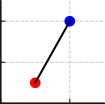
\includegraphics{images/fig3.png}\captionof{figure}{Camino más corto}
	\end{center}
	\end{minipage}
\end{minipage}
\linea
\end{lstlisting}
%

\bigskip
\linea
\begin{minipage}{1.0\textwidth}
	\begin{minipage}{0.6\textwidth}
		 \vspace{-2\baselineskip} % solo aplica para pdf
		El espacio Euclidiano es  $\R^2$, con  la métrica
		\[
		ds^2=dx^2+dy^2
		\]
		En este modelo, la distancia más corta entre dos puntos es una línea recta
	\end{minipage}\hfill\begin{minipage}{0.35\textwidth}
		\begin{center}
		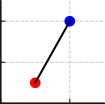
\includegraphics{images/fig3.png}\captionof{figure}{Camino más corto}
		\end{center}
	\end{minipage}
\end{minipage}
\linea


\subsection{Matrices, ecuaciones y arreglos} Make4ht traduce estos entornos sin problema. Entornos demasiado complejos, posiblemente sea mejor, insertarlos en el HTML como una imagen SVG, como se indica en  el apéndice \ref{tosvg}, o generar el equivalente HTML con IA, si se pudiera.


El código completo de  algunos ejemplos,  se puede ver en el archivo \tt{plantilla.tex}

\be
\item El código \ref{codeequnderb} muestra un ejemplo  del entorno \tt{equation}  con \tt{underbrace}


\bigskip\begin{lstlisting}[caption={\tt{equation} con \tt{underbrace}},label={codeequnderb}]
\begin{equation}
  \norm{f - L}_{\infty} = \overbrace{\abs{\frac{K_2}{2}}}^{\mathclap{\text{worst $f''(x)$ }}}\underbrace{\left(\frac{h}{2}\right)^2}_{\mathclap{\text{worst (b - a)}}}
\end{equation}
\end{lstlisting}


\begin{equation}
	\norm{f - L}_{\infty} = \overbrace{\abs{\frac{K_2}{2}}}^{\mathclap{\text{worst $f''(x)$ }}}\underbrace{\left(\frac{h}{2}\right)^2}_{\mathclap{\text{worst (b - a)}}}
\end{equation}


\item[$\bullet$]  El código \ref{codeeqcases} muestra un ejemplo  del entorno \tt{equation}  con \tt{cases}\\


%
\bigskip\begin{lstlisting}[caption={\tt{equation} y \tt{cases}},label={codeeqcases}]
\begin{equation}\label{eq:cases}
S_{i,t}=
\begin{cases}
 \begin{cases}
  [x_{i,t}=X^*, r_{i,t}=1] & \text{if  $\max\{X_{i,t}\}=X^*$} \\
  [x_{i,t}=\max\{X_{i,t}\}, r_{i,t}=0] & \text{if $\max\{X_{i,t}\} \neq X^*$}
 \end{cases}
  &\text{if $\sum_{i=1}^I u_{i,t-1}= \theta^{t-2} X^*$}\\
 \begin{cases}
  [x_{i,t}=1, r_{i,t}=1] & \hspace{\maxmin} \text{if $\min\{X_{i,t}\}=1$} \\
  [x_{i,t}=\min\{X_{i,t}\}, r_{i,t}=0] & \hspace{\maxmin} \text{if $\min\{X_{i,t}\} \neq 1$}
 \end{cases}
 &\text{otherwise}
 \end{cases}
\end{equation}
\end{lstlisting}
%

\bigskip
\begin{equation}\label{eq:cases}
	S_{i,t}=
	\begin{cases}
		\begin{cases}
			[x_{i,t}=X^*, r_{i,t}=1] & \text{if  $\max\{X_{i,t}\}=X^*$} \\
			[x_{i,t}=\max\{X_{i,t}\}, r_{i,t}=0] & \text{if $\max\{X_{i,t}\} \neq X^*$}
		\end{cases}
		&\text{if $\sum_{i=1}^I u_{i,t-1}= \theta^{t-2} X^*$}\\
		\begin{cases}
			[x_{i,t}=1, r_{i,t}=1] & \hspace{\maxmin} \text{if $\min\{X_{i,t}\}=1$} \\
			[x_{i,t}=\min\{X_{i,t}\}, r_{i,t}=0] & \hspace{\maxmin} \text{if $\min\{X_{i,t}\} \neq 1$}
		\end{cases}
		&\text{otherwise}
	\end{cases}
\end{equation}


\bigskip
Hacemos referencia a los entornos en la manera usual.\\

El código: \lstinline+En la ecuación \ref{eq:cases}, o el formato  \eqref{eq:cases}, se tiene que ...+ produce:
En la ecuación \ref{eq:cases}, o el formato  \eqref{eq:cases}, se tiene que ...\\



\item[$\bullet$] Entorno \tt{equation} con \tt{array}\\
\begin{equation*}
	{\underbrace{
			\mspace{3mu}
			\left(\begin{array}{c} b_1 \\ b_2 \\ b_3 \\ \vdots \\ b_n \end{array}\right)
			\mspace{3mu}
		}_{\textstyle\mathstrut\boldsymbol{b}}} =
	{\underbrace{
			\left(\begin{array}{*{5}{c}}
				s_{11} & s_{12} & s_{13} & \dots & s_{1n} \\
				s_{21} & s_{22} & s_{23} & \dots & s_{2n} \\
				s_{31} & s_{32} & s_{33} & \dots & s_{3n} \\
				\vdots & \vdots & \vdots & \ddots& \vdots \\
				s_{n1} & \dots  & \dots  & \dots & s_{nn}
			\end{array}\right)
		}_{\textstyle\mathstrut\boldsymbol {S}}}
	\mspace{3mu}\cdot
	{\underbrace{
			\mspace{3mu}
			\left(\begin{array}{c} a_1 \\ a_2 \\ a_3 \\ \vdots \\ a_n \end{array}\right)
			\mspace{3mu}
		}_{\textstyle\mathstrut\boldsymbol{a}}}
\end{equation*}

\item[$\bullet$] Entorno \tt{pmatrix} con \tt{block}\\

\[
\underbrace{
	\begin{pmatrix}
		1 & \smash[b]{\underbrace{1 \cdots 1}_{k}} \\
		&& 1 & \smash[b]{\underbrace{1 \cdots 1}_{k}} \\
		&&&& \ddots \\
		&&&&& 1 & \underbrace{1 \cdots 1}_{k}
	\end{pmatrix}
}_{T}
\]

\ee


\subsection{Listas de ejercicios}\label{listaejercicios} El documento \tt{plantilla.tex} usa el paquete \tt{exsheets} para manejar listas de ejercicios al compilar con PDFLaTeX. En el preámbulo podremos ver el código que muestra \ref{codeexs}


\bigskip\begin{lstlisting}[caption={Habilitar \tt{exsheets} para PDFLaTeX},label={codeexs}]
\ifdefined\HCode % Paquete de ejercicios exsheets,no soportado por Make4ht
\else % compila PDFLatex
\usepackage[counter-format=se.qu,counter-within=section]{exsheets}
\DeclareTranslation{english}{exsheets-exercise-name}{\textcolor{tverde}{Ejercicio}}
\DeclareTranslation{english}{exsheets-question-name}{\textcolor{tverde}{Pregunta}}
 \DeclareTranslation{english}{exsheets-solution-name}{\textcolor{tverde}{Solución}}
\SetupExSheets{
	question/pre-body-hook = {\normalfont},
	solution/pre-hook = {\par\medskip},
}
\fi
\end{lstlisting}


Cuando compilamos con Make4ht, usamos el mismo código que en PDFLaTeX, solo que en el preámbulo se han definido los comandos para que PDFLaTeX lo interprete de una forma y Make4ht de otra, de tal manera que tengamos listas de ejercicios en ambos ambientes usando el mismo código.

\be
\item \lstinline+\hejersol{}{}+. Este comando lo ignora PDFLaTeX y Make4ht lo convierte en un enunciado con un botón Ver/Ocultar, para ver la respuesta en el renglón que sigue.

\item \lstinline+\ejersol{}{}+.

Este comando funciona para PDFLaTeX y Make4ht. PDFLaTeX lo convierte en un ejercicio normal y, para ver las soluciones,  se pone al final del documento

\lstinline+\solopdf{ \section*{Respuestas} \printsolutions }{} +
\ee


Si compilamos con  Make4ht, \lstinline+\ejersol{}{}+ se convierte en  \lstinline+\hejersol{}{}+.
La idea es que a veces, un mismo ejercicio tiene un enunciado en el PDF, digamos con una figura fija por ejemplo, mientras que el enunciado en HTML no necesita la figura porque viene con otra cosa, por ejemplo un script.


\textbf{Ejemplo.} En el código \ref{codelejer} se muestra una lista de ejercicios. La salida en PDF corresponde al formato del paquete \tt{exsheets}, la salida en HTML es una lista de enunciados con un botón para ver/ocultar la respuesta. La \tt{plantilla.tex} contiene el código para insertar el script que gobierna el botón y su acción.

\bigskip
\bigskip\begin{lstlisting}[caption={Lista de ejercicios},label={codelejer}]
% Ejercicio 1:
\hejersol{Resuelve para $x$: $\frac{2}{3}x + 5 = 10$}{La solución es $x = \frac{15}{2}$}\\
% Ejercicio 2:
\ejersol{Calcula el área de un cuadrado de lado 3 cm}{$9\ \text{cm}^2$}\\
% Ejercicio 3:
\ejersol{Deriva $f(x) = 3x^2 + 2x - 1$}{$f'(x) = 6x + 2$}\\
% Ejercicio 4:
\ejersol{Simplifica $\sin^2 \theta + \cos^2 \theta$}{$1$}\\
% Ejercicio 5:  Solo PDFLaTeX
\solopdf{\ejersol{Calcula la velocidad final si $v_0=10\,m/s$,
        $a=2\,m/s^2$ y $t=3\,s$}{$16\,m/s$}
        }\\
% Ejercicio 6: Solo Make4ht
\solomk{\hejersol{Encuentra la energía cinética de un objeto de 5 kg
           moviéndose a 4 m/s}{$40\,J$}
        }\\
% Ejercicio 7:  Solo Make4ht
\hejersol{Halla la corriente si $V=12\,V$ y $R=4\,\Omega$}{$3\,A$}\\

% Al finaldel documento: \solopdf{ \section*{Respuestas} \printsolutions }{}
\end{lstlisting}

\solopdf{En la Figura \ref{desplegable} podemos ver el desplegable con la solucón en el HTML}


% Ejercicio 1: Álgebra
\ejersol{Resuelve la ecuación $\frac{2}{3}x + 5 = 10$
}{La solución es $x = \frac{15}{2}$}

\solopdf{
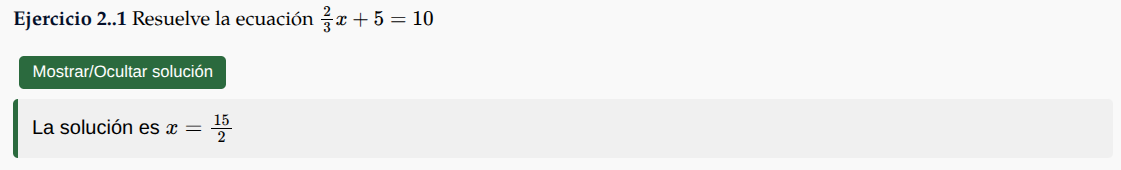
\includegraphics[width=1\textwidth]{images/botonVerOcultar.png}
\captionof{figure}{Desplegable HTML,  para ejercicio y solución}\label{desplegable}
}

% Ejercicio 2: Geometría
\ejersol{Calcular el área de un cuadrado de lado 3 cm}{$9\ \text{cm}^2$}

% Ejercicio 3: Cálculo
\ejersol{Derivar $f(x) = 3x^2 + 2x - 1$}{$f'(x) = 6x + 2$}

% Ejercicio 4: Trigonometría
\ejersol{Simplificar $\sin^2 \theta + \cos^2 \theta$}{$1$}

% 1. Cinemática: Solo PDFLaTeX
\solopdf{\ejersol{Calcula la velocidad final si $v_0=10\,m/s$, $a=2\,m/s^2$ y $t=3\,s$}{$16\,m/s$}
}

% 2. Energía: Solo Make4ht
\solomk{ \ejersol{Encuentra la energía cinética de un objeto de 5 kg moviéndose a 4 m/s}{$40\,J$} }

% 3. Electricidad: Solo Make4ht
\hejersol{Halla la corriente si $V=12\,V$ y $R=4\,\Omega$}{$3\,A$}

\subsection{Tabla de contenidos: Ver/Ocultar} La tabla de contenidos en el PDF
se obtiene con \lstinline+\tableofcontents+. Make4ht compila \lstinline+\tableofcontents+ y genera una tabla de contenidos adecuada para el HTML.\\

La plantilla incluye un botón \lstinline+\cejilla{#1}{#2}+ que abre y cierra una ventana (un "desplegable"). Lo podemos usar, entre muchas cosas, para desplegar  el "Contenido" en la \tt{plantilla.html}. Se requiere un script \tt{cejilla.js} y un archivo \tt{cejilla.css} que ya están en las carpetas CSS  y JS. El código \ref{codebtc} muestra la manera de habilitar el botón. \solopdf{ La Figura \ref{fig:codebtc} es una vista de cómo se ve en el HTML}.


\bigskip\begin{lstlisting}[caption={plantilla.tex},label={codebtc}]
\begin{document}
\maketitle
\solopdf{\tableofcontents} % Genera la tabla de contenidos
% Desplegable de propósito general
\solomk{\cejilla{Tabla de contenidos}{\tableofcontents}}
\end{lstlisting}

\solopdf{\begin{center}
\wref{RevistaDigital_V25_n2_2025_Mora.html\#ancla-botonTablaContenidos}{
 
\includegraphics[width=\textwidth]{images/botontcontenidos.png}}
 \captionof{figure}{Botón para desplegar la tabla de contenidos}\label{fig:codebtc}
\end{center}
}


\solomk{
\cejilla{Tabla de contenidos}{%
   \tableofcontents
}}


\section{Entornos definición, teorema, ejemplo, etc.}
La plantilla tiene varios entornos ya configurados para que compilen bien con Make4ht.
Agregar nuevos entornos posiblemente requiera agregar nuevo código al archivo de configuración \tt{config.cfg} (ver sección \ref{sec:configurarmake4ht}). Lo recomendable es usar los modelos que ya están en este archivo. Si usa IA para configurar algún nuevo entorno, lo mejor es indicarle que genere  código siguiendo esos modelos ya probados y avalados por la documentacion más reciente.

Para el PDF d ela plantilla, las cosas de  dise\~no  de cada entorno, como bordes, color, color de fondo, etc. se puede modificar en \tt{WebPreambuloyEntornos.tex}.

Modificar el dise\~no de cada entorno, para la salida HTML,
requiere modificar entre otras cosas, el  \lstinline+\Css{...}+ del entorno en el  archivo \tt{config.cfg}. Por ejemplo, el código \ref{codeedef} muestra parte  del dise\~no del entorno para las definiciones (además se debe controlar los cierres de etiquetas y los entornos \tt{minipage} dentro de las definiciones).


\bigskip\begin{lstlisting}[caption={Parte del dise\~no para el entorno "definicion" (ya implementado).},label={codeedef}]
% Archivo config.cfg
\Css{% No dejar renglones en blanco y "escapar" \# y \%
 .definicion {
   background-color: rgb(251, 251, 250);
   border-left: 4pt solid rgb(255, 20, 147);
   margin: 20pt 0;
   padding: 0pt 4pt 0 4pt;
   overflow: auto;
   clear: both;
	}
  .definicion-title {
   color: rgb(255, 20, 147);
   font-weight: bold;
   margin-bottom: 0.5em;
   display: block;
}																									\end{lstlisting}



A continuación tenemos una lista de entornos con ejemplos.

\be % Entornos
\item Definiciones. El código \ref{codeudef}  muestra el formato general de una definición.

%
\bigskip\begin{lstlisting}[caption={Una definición},label={codeudef}]
\label{def:defi1}
\begin{definicion}[nombre-opcional]
 Contenido...
\end{definicion}
\end{lstlisting}
%

\bigskip
$\bullet$\; Una definción con nombre.\\

\label{def:defi1}
\begin{definicion}[Envoltura Convexa]
Sea $S \subset \mathbb{R}^n$  un conjunto de puntos. La {\it envoltura convexa} de $S$, denotada por
 $\text{Conv}(S)$, es el conjunto convexo más pequeño que contiene a $S$. Formalmente:

\[
\text{Conv}(S) = \left\{ \sum_{i=1}^{k} \lambda_i x_i \;\middle|\; x_i \in S,\; \lambda_i \geq 0,\; \sum_{i=1}^{k} \lambda_i = 1,\; k \in \mathbb{N} \right\}
\]

Es decir, \( \text{Conv}(S) \) está formado por todas las combinaciones convexas finitas de puntos de $ S $.
\end{definicion}
%

\bigskip
Bien, ahora podemos hacer referencia con usual con  \lstinline+\ref+: En la Definición \ref{def:defi1}...\\

\bigskip
%-----------------------------------------------------------------------------
\solomk{
	\begin{minipage}[t]{1.0\textwidth}
	\begin{minipage}{0.65\textwidth}Sean \( A = (1,1) \), \( B = (2,4) \), \( C = (4,0) \).
		El punto \( P = (3,1) \) está dentro del triángulo pues:
		\[
		P = \tfrac{1}{4}A + \tfrac{1}{4}B + \tfrac{1}{2}C.
		\]
		Como \( \lambda_1 = \tfrac{1}{4},\, \lambda_2 = \tfrac{1}{4},\, \lambda_3 = \tfrac{1}{2} \), y \( \lambda_i \geq 0 \), entonces se concluye que \( P \in \text{Conv}\{A,B,C\} \).
	\end{minipage}\hfill\begin{minipage}{0.28\textwidth}
	\begin{center}
	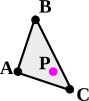
\includegraphics[scale=0.6]{images/fig2.svg}\captionof{figure}{
		$\triangle ABC$}\label{ej:ejemplo20}
		\end{center}
	\end{minipage}
\end{minipage}
}
\insertarhtml{<hr style="height:1px;border-width:0;color:gray;background-color:gray">}

%-----------------------------------------------------------------------------


\bigskip
$\bullet$\; Una definición con \tt{minipage} y una nota \lstinline+\footnote{...}+

\bigskip
\solopdf{% PDFLaTeX->pdf
\begin{definicion}[Modelo para Geometría Hipérbolica]
	\begin{minipage}[t]{1.0\textwidth}
		\begin{minipage}{0.65\textwidth}
Un modelo para la geometría hiperbólica es el \tt{semiplano superior}
\[
\mathbb{H} = \left\{ (x, y) \in \mathbb{R}^2 \,\middle|\, y > 0 \right\}
\]
equipado con la métrica
\[
ds^2 = \frac{dx^2 + dy^2}{y^2}.
\]

Al conjunto $\mathbb{H}$ se le llama \tt{semiplano superior de Poincaré}.
\footnote{En honor al gran matemático francés que lo descubrió.}
		\end{minipage}\hfill\begin{minipage}{0.32\textwidth}
		\centering
			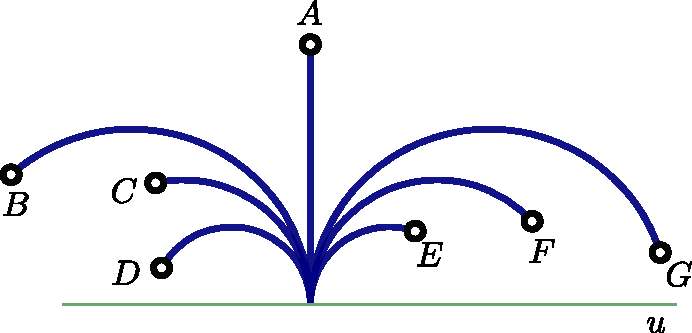
\includegraphics[scale=0.4]{images/paralelasPoincare.pdf}
			\captionof{figure}{Rectas paralelas}\label{ej:ejemplo1}
		\end{minipage}
	\end{minipage}
\end{definicion}
}
\solomk{% Make4ht -> html
\begin{definicion}[Modelo para Geometría Hipérbolica]
	\begin{minipage}[t]{1.0\textwidth}
		\begin{minipage}{0.65\textwidth}
Un modelo para la geometría hiperbólica es el \tt{semiplano superior}
\[
\mathbb{H} = \left\{ (x, y) \in \mathbb{R}^2 \,\middle|\, y > 0 \right\}
\]
equipado con la métrica
\[
ds^2 = \frac{dx^2 + dy^2}{y^2}. \tag{C}
\]

Al conjunto $\mathbb{H}$ se le llama \tt{semiplano superior de Poincaré}.\footnote{En honor al gran matemático francés que lo descubrió.}
		\end{minipage}\hfill\begin{minipage}{0.28\textwidth}
		\centering
			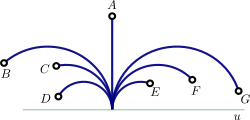
\includegraphics{images/paralelasPoincare.svg}
			\captionof{figure}{Rectas paralelas}\label{ej:ejemplo1}
		\end{minipage}
	\end{minipage}
\end{definicion}
}


\bigskip
\item Teoremas. El código \ref{codeuteo}  muestra el formato general de un teorema.\\

%
\bigskip\begin{lstlisting}[caption={Un teorema},label={codeuteo}]
\label{teo:teo1}
\begin{teorema}[nombre-opcional]
		Contenido...
\end{teorema}
\end{lstlisting}
%

\bigskip
$\bullet$\; Teorema con nombre.\\


\label{teo:teo1}
\begin{teorema}[Parametrización de un triángulo]
Sean $A,B,C \in \R^2$ no colineales entonces existen $t,s,w$ únicos tales que
$$\triangle ABC=
\{t A + s B + w C,
\quad \text{donde } t,s,w\geq 0, \quad
t+s+w = 1\}
$$
\end{teorema}

\bigskip
$\bullet$\; El código \ref{codeuteodem} muestra un teorema con demostración. Usamos  un entorno \tt{caja} que ya está configurado. Es una caja simple, con fondo blanco pero tiene atributos bien definidos en la configuración para la  traducción a HTML.\\


\bigskip
\bigskip\begin{lstlisting}[caption={Un teorema con demostración},label={codeuteodem}]
\label{teo:teo2}
\begin{teorema}[La recta es el camino más corto]
...
\begin{caja}[Demostración.]
...
\end{caja}
\end{teorema}
\end{lstlisting}


\bigskip
\label{teo:teo2}
\begin{teorema}[La recta es el camino más corto]
En el plano euclidiano $\mathbb{R}^2$ con la métrica usual, el camino más corto entre dos puntos $A$ y $B$ es el segmento de recta que los une.
%
\begin{caja}[Demostración]
Sea \(x\) un número real arbitrario.
Sea $\gamma(t) = (x(t), y(t))$ una curva suave que une dos puntos $A$ y $B$ en el intervalo $[a, b]$. Su longitud es:
\[
L[\gamma] = \int_a^b \sqrt{x'(t)^2 + y'(t)^2}\, dt.
\]

Aplicamos la desigualdad de Cauchy–Schwarz:
\[
L[\gamma] \geq \sqrt{(x(b) - x(a))^2 + (y(b) - y(a))^2},
\]
con igualdad si y solo si $\gamma'(t)$ es constante y paralelo al vector $B - A$, es decir, si $\gamma$ es una recta.

Por lo tanto, la longitud mínima se alcanza exactamente cuando $\gamma$ es el segmento de recta entre $A$ y $B$.\hfill\qedsymbol
\end{caja}
%
\end{teorema}



\bigskip
En el HTML También podemos usar el comando \lstinline+\cejilla{demostracion}{...}+ para ocultar latdemostración con en una ventana desplegable, como se muestra en el código \ref{codeuteodemb}


\bigskip
\bigskip\begin{lstlisting}[caption={Un teorema y demostración desplegable},label={codeuteodemb}]
\solomk{
\label{teo:teo2}
\begin{teorema}[La recta es el camino más corto]
En el plano euclidiano $\mathbb{R}^2$
...
\end{teorema}
% Desplegable
\cejilla{Demostración}{
\begin{caja}
Sea \(x\) un número real arbitrario.
...
\end{caja}
}%cejilla
}%solomk
\end{lstlisting}


\bigskip
\solomk{
\label{teo:teo2a}
\begin{teorema}[La recta es el camino más corto]
En el plano euclidiano $\mathbb{R}^2$ con la métrica usual, el camino más corto entre dos puntos $A$ y $B$ es el segmento de recta que los une.
\end{teorema}
\cejilla{Demostración}{
\begin{caja}
Sea \(x\) un número real arbitrario.
Sea $\gamma(t) = (x(t), y(t))$ una curva suave que une dos puntos $A$ y $B$ en el intervalo $[a, b]$. Su longitud es:
\[
L[\gamma] = \int_a^b \sqrt{x'(t)^2 + y'(t)^2}\, dt.
\]

Aplicamos la desigualdad de Cauchy–Schwarz:
\[
L[\gamma] \geq \sqrt{(x(b) - x(a))^2 + (y(b) - y(a))^2},
\]
con igualdad si y solo si $\gamma'(t)$ es constante y paralelo al vector $B - A$, es decir, si $\gamma$ es una recta.

Por lo tanto, la longitud mínima se alcanza exactamente cuando $\gamma$ es el segmento de recta entre $A$ y $B$.\hfill\qedsymbol
\end{caja}
}
}%%solomk



\bigskip
 \item El código \ref{codeuej}  muestra el formato general de un  ejemplo ilustrativo.

\bigskip
  \bigskip\begin{lstlisting}[caption={Un ejemplo},label={codeuej}]
\label{ej:ejemplo1}
\begin{ejemplo}[nombre-opcional]
 % Enunciado
\end{ejemplo}
\end{lstlisting}


\bigskip
\textbf{Ejemplo:} El código,  \ref{codeuejsol} muestra un ejemplo con un entorno \tt{minipage}\\

 \bigskip\begin{lstlisting}[caption={Un ejemplo con solución},label={codeuejsol}]
\solopdf{ % PDFLaTeX -> pdf
\label{ej:ejemplo1}
\begin{ejemplo}[Punto dentro del triángulo]
   \begin{minipage}{0.7\textwidth}
	  Sean \( A = (1,1) \), \( B = (2,4) \), \( C = (4,0) \).
        ...
   \end{minipage}\hfill\begin{minipage}{0.2\textwidth}
       ...
    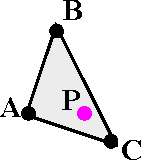
\includegraphics[scale=0.7]{images/fig2.pdf}
  \end{minipage}
\end{ejemplo}
 }
 \solomk{  % Make4ht -> html
\label{ej:ejemplo1}
\begin{ejemplo}[Punto dentro del triángulo]
   \begin{minipage}{0.7\textwidth}
	  Sean \( A = (1,1) \), \( B = (2,4) \), \( C = (4,0) \).
        ...
   \end{minipage}\hfill\begin{minipage}{0.2\textwidth}
       ...
   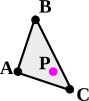
\includegraphics[scale=0.7]{images/fig2.svg}
   \end{minipage}
   \end{ejemplo}
\end{ejemplo}
}
 \end{lstlisting}


  \bigskip
   \solopdf{ %pdf
  	\label{ej:ejemplo1}
  	\begin{ejemplo}[Punto dentro del triángulo]
  		\begin{minipage}{0.65\textwidth}
  		Sean \( A = (1,1) \), \( B = (2,4) \), \( C = (4,0) \).
 		El punto \( P = (3,1) \) está dentro del triángulo $\triangle ABC$ pues, como este triágulo es un conjunto comvexo y
  			\[
  			P = \tfrac{1}{4}A + \tfrac{1}{4}B + \tfrac{1}{2}C.
  			\]
  			 entonces se concluye que \( P \in \text{Conv}\{A,B,C\} =\triangle ABC \).
  		\end{minipage}\hfill\begin{minipage}{0.28\textwidth}
  			\centering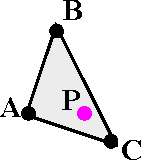
\includegraphics{images/fig2.pdf}\captionof{figure}{
  				\(\triangle ABC\) y \(P\)}\label{fig:ejemplo2}
  		\end{minipage}
  	\end{ejemplo}
 %
 }
 \solomk{  % html---------------------------------
 %
 	\label{ej:ejemplo1}
  	\begin{ejemplo}[Punto dentro del triángulo]
  	\begin{minipage}{1.0\textwidth}
  		\begin{minipage}{0.65\textwidth}
  		Sean \( A = (1,1) \), \( B = (2,4) \), \( C = (4,0) \).
 		El punto \( P = (3,1) \) está dentro del triángulo $\triangle ABC$ pues, como este triágulo es un conjunto comvexo y
  			\[
  			P = \tfrac{1}{4}A + \tfrac{1}{4}B + \tfrac{1}{2}C.
  			\]
  			 entonces se concluye que \( P \in \text{Conv}\{A,B,C\} =\triangle ABC \).
  		\end{minipage}\hfill\begin{minipage}{0.28\textwidth}
  			\begin{center}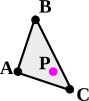
\includegraphics{images/fig2.svg}\captionof{figure}{
  				\(\triangle ABC\) y \(P\)}\label{fig:ejemplo2}
  				\end{center}
  		\end{minipage}
	\end{minipage}
  	\end{ejemplo}
 } %html---------------------------------


 \bigskip
También podemos editar un ejemplo con solución, usando el entorno \lstinline+\begin{caja}[Solución]+.\\


\begin{ejemplo}[Punto fuera del triángulo]%
		Sean \( A = (1,1) \), \( B = (2,4) \), \( C = (4,0) \). Sea \( P = (3,4) \).
		Verifique que \( P \) está fuera del triángulo \( \triangle ABC \).\\
%solucion
\begin{caja}[Solución]
		Resolviendo el sistema \(3\times 3\)
		\[
		P = t A + s B + w C,\quad t + s + w = 1,
		\]
		obtenemos la única solución \( t=-1, \, s=2,\, w=0 \), y como uno de los coeficientes es negativo,
		\( P \notin \text{Conv}\{A,B,C\} =\triangle ABC\). \hfill \qedsymbol
\end{caja}
\end{ejemplo}
 \ee % Fin entornos

 \bigskip
En esta plantilla se han definido más entornos. El dise\~no se puede modoficar tanto en el archivo \tt{WebPreambuloyEntornos.tex}(paraPDFLaTeX) como en el archivo de configuración \tt{config.cfg} (para Make4ht). La lista de entornos es\\



    \begin{enumerate}
        \item \lstinline+\ObjetivoGeneral{...}+
        \item \lstinline+\ObjetivosEspecificos{...}+
        \item \lstinline+\resumen{...}+
        \item \lstinline+\palabrasclave{...}+
        \item \lstinline+\abstract{...}+
        \item \lstinline+\keywords{...}+
        \item \lstinline+\begin{definicion}...\end{definicion}+
        \item \lstinline+\begin{teorema}...\end{teorema}+
        \item \lstinline+\begin{ejemplo}...\end{ejemplo}+
        \item \lstinline+\begin{corolario}...\end{corolario}+
        \item \lstinline+\begin{proposicion}...\end{proposicion}+
        \item \lstinline+\begin{lema}...\end{lema}+
        \item \lstinline+\begin{caja}...\end{caja}+
        \item \lstinline+\begin{axioma}...\end{axioma}+
        \item \lstinline+\begin{actividad}...\end{actividad}+
        \item \lstinline+\begin{notahistorica}...\end{notahistorica}+
        \item \lstinline+\begin{problema}...\end{problema}+
        \item \lstinline+\begin{ejercicio}...\end{ejercicio}+
        \item \lstinline+\begin{proyecto}...\end{proyecto}+
        \item \lstinline+\begin{aplicacion}...\end{aplicacion}+
    \end{enumerate}




    \subsection{Un problema de optimización: Ejercicio y respuesta.}

El área $A$ del trapecio isósceles inscrito en la parte superior de una circunferencia de ecuación $x^2+y^2=16$ se puede escribir en función de la base menor, de longitud $2a$:

\[
A(a) = \frac{(B + b) \cdot h}{2} = \frac{(8 + 2a) \cdot \sqrt{16 - a^2}}{2}
\]

Si $a=0$, tendríamos un triángulo de área $8ul^2$. Si nos interesa el valor de $a$ para que el trapecio tenga área máxima, debemos resolver $A'(a)=0$ y, formalmente, verificar que se trata de un máximo global.\\

\solopdf{%PDFLaTeX-> pdf
En la  Figura \ref{optrapecio} se ilustra la situación.\\
}


\solomk{
% Make4ht->html
En el siguiente script podemos, con el deslizador, hacer que $a$ tome los  valores permitidos, es decir, $a\in[0,4]$. En la tabal podemos ver como varía el área y en el gráfico de la derecha vemos que hay un valor de $a$ en que el área es máxima. Y queremos calculor el valor exacto de $a$ en el que el área del trapecio es máxima.
}

El código \ref{code1popt} muestra como insertar en el HTML la página \tt{.html} completa.\\


\bigskip\begin{lstlisting}[caption={Problema de optimización},label={code1popt}]
\solomk{
\VentanayAbrirVentanaIndependiente
  {trapecioOptimizacion.html}  % #1 URL
  {800}                                % #2 ancho iframe (px)
  {500}                                % #3 alto iframe (px)
  {70}                                 % #4 ancho popup (%)
  {80}                                 % #5 alto popup (%)
  {Problema de  optimización}                 % #6 título
  {Puedes interactuar aquí o abrirla en ventana aparte}  % #7
  }%solomk
\end{lstlisting}

\solomk{
 \HCode{<div class="opt-trap-container" id="ancla-proboptimizacion">}
 \VentanayAbrirVentanaIndependiente
  {trapecioOptimizacion.html}  % #1 URL
  {800}                                % #2 ancho iframe (px)
  {500}                                % #3 alto iframe (px)
  {70}                                 % #4 ancho popup (%)
  {80}                                 % #5 alto popup (%)
  {P}                 % #6 título
  {Puedes interactuar aquí o abrirla en ventana aparte}  % #7
 \HCode{</div>}
 }


  \bigskip
\solopdf{ %PdfLaTeX->pdf
En el HTML tendríamos algo como lo que muestra la Figura \ref{optrapecio}
\begin{center}
\wref{RevistaDigital_V25_n2_2025_Mora.html\#ancla-proboptimizacion}{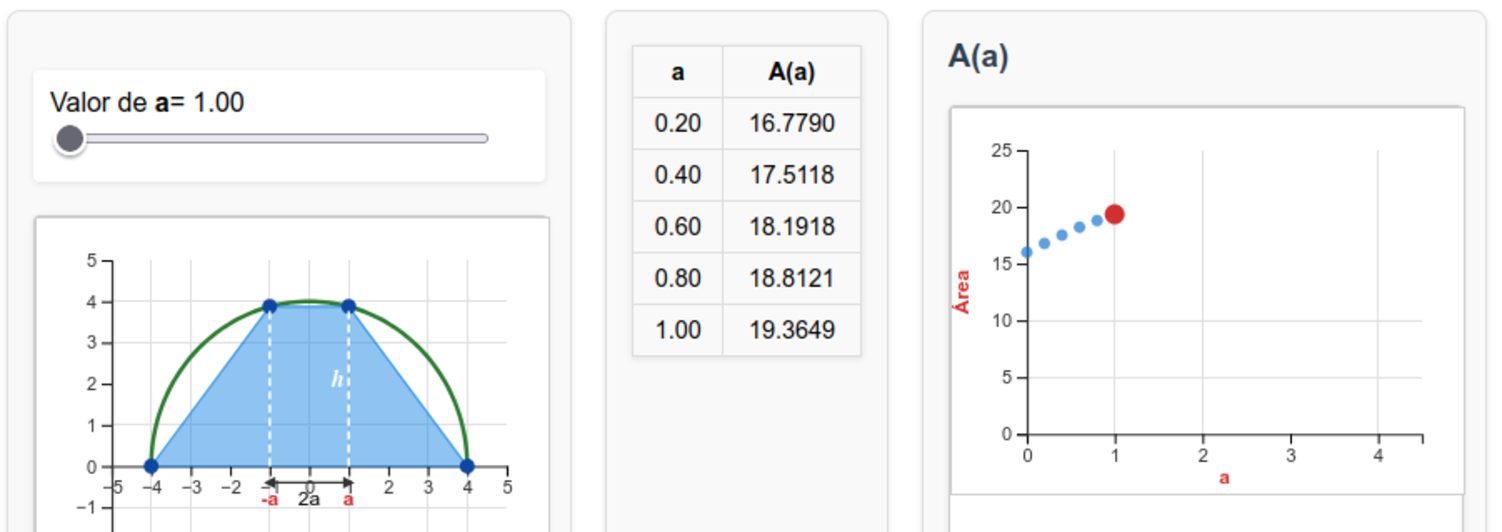
\includegraphics[scale=0.55]{images/scriptopttrapecio.pdf}}¨
\captionof{figure}{Script en \tt{plantilla.html}}\label{optrapecio}
\end{center}
}


\subsubsection{Ejemplos.}

\fvnp{Distribución Normal.} El código \ref{codedngeog} muestra como insertar un applet de Geogebra para visualizar el cálculo de áreas en la \href{https://www.geogebra.org/m/rZ7NHCsS}{Distribución Normal}.\\

\solopdf{%PDFLaTeX -> pdf
En el documento \tt{plantilla.html} aparece el botón para abrir o cerrar la ventana, con el applet de Geogebra, como se muestra en la Figura \ref{scriptdistribNormal}
\begin{center}
\wref{RevistaDigital_V25_n2_2025_Mora.html\#ancla-dngeogebra}{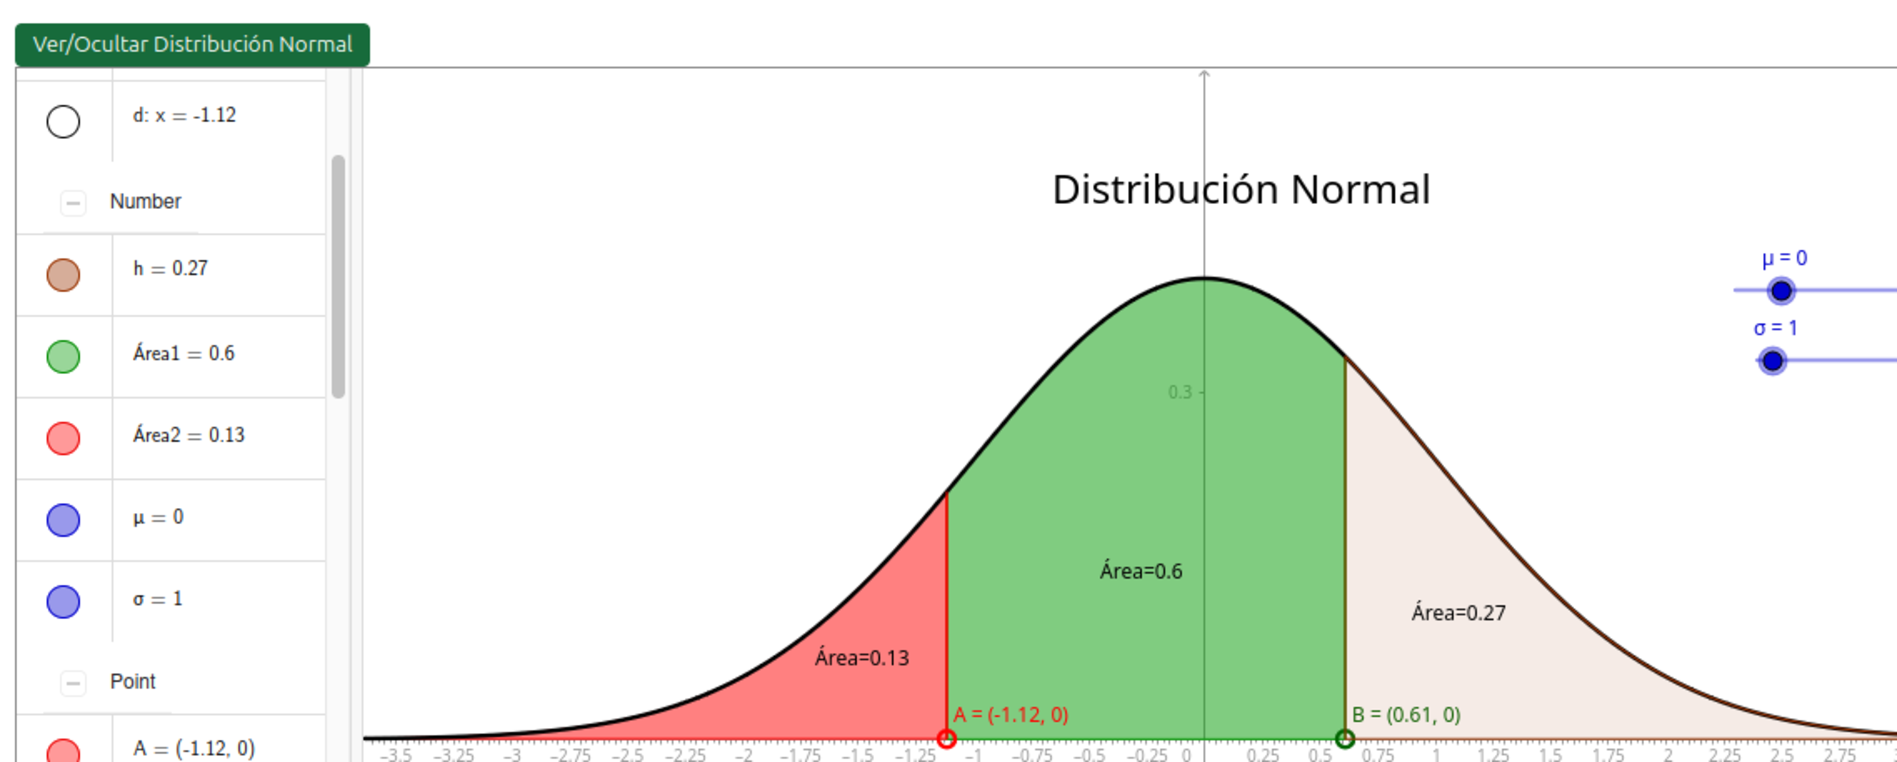
\includegraphics[scale=0.4]{images/scriptdistribNormal.pdf}}
\captionof{figure}{Script en \tt{plantilla.html}}\label{scriptdistribNormal}
\end{center}
}

 \bigskip\begin{lstlisting}[caption={Distribución Normal},label={codedngeog}]
\solomk{
\cejilla{Geogebra: Distribución Normal}{
\insertarhtml{%
    <iframe scrolling="no" title="Distribución Normal" src="https://www.geogebra.org/material/iframe/id/rZ7NHCsS/width/1366/height/609/border/888888/sfsb/true/smb/false/stb/false/stbh/false/ai/false/asb/false/sri/false/rc/false/ld/false/sdz/false/ctl/false" width="900px" height="402px" style="border:0px;"></iframe>
}
}%insertarhtml
}%solomk
 \end{lstlisting}
\solomk{
\cejilla{Geogebra: Distribución Normal}{
\insertarhtml{% ventana1
        <iframe scrolling="no" title="Distribución Normal" src="https://www.geogebra.org/material/iframe/id/rZ7NHCsS/width/1366/height/609/border/888888/sfsb/true/smb/false/stb/false/stbh/false/ai/false/asb/false/sri/false/rc/false/ld/false/sdz/false/ctl/false" width="900px" height="402px" style="border:0px;"></iframe>
}
}%insertarhtml
}%solomk






\bigskip
\fvnp{Tabla de Frecuencias.} Este es otro ejemplo que tomamos de la página de \href{https://www.geogebra.org/materials}{Recursos}. Es un applet de Geogebra con una actividad interactiva con \href{https://www.geogebra.org/m/kOdi0K5V}{tablas de frecuencias} para el  tema de Estadística.\\

El código \ref{codegeotfrec} muestra como insertar en el HTML

\bigskip
\bigskip\begin{lstlisting}[caption={Tabla de frecuencias},label={codegeotfrec}]
\solomk{
\cejilla{Geogebra: Tabla de frecuencias}{
\insertarhtml{% ventana1
  <iframe scrolling="no" title="Tabla de frecuencias" src="https://www.geogebra.org/material/iframe/id/sxG0ihm3/width/900/height/400/border/888888/sfsb/true/smb/false/stb/false/stbh/false/ai/false/asb/false/sri/false/rc/true/ld/false/sdz/false/ctl/false" width="800px" height="400px" style="border:0px;"> </iframe>
}
}%insertarhtml
}%solomk
\end{lstlisting}


\solomk{
\cejilla{Geogebra: Tabla de frecuencias}{
\insertarhtml{% ventana1
  <iframe scrolling="no" title="Tabla de frecuencias" src="https://www.geogebra.org/material/iframe/id/sxG0ihm3/width/900/height/400/border/888888/sfsb/true/smb/false/stb/false/stbh/false/ai/false/asb/false/sri/false/rc/true/ld/false/sdz/false/ctl/false" width="800px" height="400px" style="border:0px;"> </iframe>
}
}%insertarhtml
}%solomk



\subsection{Incrustar videos}
De manera similar a como incrustamos applets de Geogebra, también incrustamos videos de YouTube, u otra fuente, en la salida HTML de nuestro documento \tt{.tex}. Usamos el mismo comando \lstinline+\cejilla{}{}+.\\

En el video de YouTube que nos interesa, hacemos click en "Compartir" y hacemos click en "Incrustar" y tomamos el código
\lstinline+<iframe ...>...</iframe>+ y lo insertamos en nuestro HTML.

\subsubsection*{Ejemplo.} \fvnp{El determinante | Esencia del álgebra lineal, capítulo 5.} El canal \href{https://youtube.com/@3blue1brownespanol?si=KPplnrHalBSjb1pB}{3Blue1Brown} tiene como meta usar animaciones para aclarar y motivar temas complejos. Hemos elegido para este ejemplo, el \href{https://youtu.be/yt3eoYvGel0?si=2izQPKrVWe4IvgPM}{capítulo 5} sobre determinantes.\\

El video lo podemos incluir en el HTML con nuestro comando \lstinline+\cejilla{}{}+ o podemos pedir a la IA un archivo \tt{.html} "responsivo" y con otras facetas adecuadas para celular, en este caso usamos el comado \lstinline+\VentanayAbrirVentanaIndependiente+\\


En el primer caso, el Código \ref{codevyoutube} muestra como insertar el video en el HTML

\bigskip
\bigskip\begin{lstlisting}[caption={El determinante: Video de YouTube},label={codevyoutube}]
% Esto no abre desde  una PC, debe estar en un sitio web
\insertarhtml{
\solomk{
\cejilla{Video: Determinantes}{
\insertarhtml{
<iframe width="560" height="315"
  src="https://www.youtube-nocookie.com/embed/yt3eoYvGel0"
  frameborder="0"
  allow="accelerometer; autoplay; clipboard-write; encrypted-media; gyroscope; picture-in-picture; web-share"
  allowfullscreen>
</iframe>
}
}%cejilla
}%solomk
\end{lstlisting}


\solomk{
\cejilla{Video: Determinantes}{
\insertarhtml{
<iframe width="560" height="315"
  src="https://www.youtube-nocookie.com/embed/yt3eoYvGel0"
  frameborder="0"
  allow="accelerometer; autoplay; clipboard-write; encrypted-media; gyroscope; picture-in-picture; web-share"
  allowfullscreen>
</iframe>
}
}%cejilla
}%solomk

\bigskip
La otra opción se muestra en el  Código \ref{codeVideoB} \\

\bigskip
\bigskip\begin{lstlisting}[caption={Video sobre determinantes},label={codeVideoB}]
\solomk{
\VentanayAbrirVentanaIndependiente
  {Determinantes.html}  % #1 URL
  {800}                                % #2 ancho iframe (px)
  {500}                                % #3 alto iframe (px)
  {70}                                 % #4 ancho popup (%)
  {80}                                 % #5 alto popup (%)
  {Video: Determinantes}                 % #6 título
  {Puedes interactuar aquí o abrirla en ventana aparte}  % #7
  }%solomk
\end{lstlisting}

\bigskip
\solomk{
\VentanayAbrirVentanaIndependiente
  {Determinantes.html}  % #1 URL
  {800}                                % #2 ancho iframe (px)
  {500}                                % #3 alto iframe (px)
  {70}                                 % #4 ancho popup (%)
  {80}                                 % #5 alto popup (%)
  {Determinantes}                 % #6 título
  {Puedes interactuar aquí o abrirla en ventana aparte}  % #7
  }%solomk

%
\begin{thebibliography}{9}

	\bibitem{bootstrap}
	BootstrapMade. (2023). \textit{BootstrapMade: Free and premium Bootstrap templates}. BootstrapMade. \url{https://bootstrapmade.com/}

	\bibitem{bmake4ht}
	Hoftich, M. (2024). \textit{TeX4ht Documentation by TeX4ht Project}. \url{https://www.kodymirus.cz/tex4ht-doc/tex4ht-doc.html}

	\bibitem{denlinger}
	Denlinger, C. G. (2010). \textit{Elements of real analysis}. Jones \& Bartlett Publishers.



\end{thebibliography}

%

\end{document}












